\def\year{2021}\relax
%File: formatting-instructions-latex-2021.tex
%release 2021.1
\documentclass[letterpaper]{article} % DO NOT CHANGE THIS
\usepackage{aaai21}  % DO NOT CHANGE THIS
\usepackage{times}  % DO NOT CHANGE THIS
\usepackage{helvet} % DO NOT CHANGE THIS
\usepackage{courier}  % DO NOT CHANGE THIS
\usepackage[hyphens]{url}  % DO NOT CHANGE THIS
\usepackage{graphicx} % DO NOT CHANGE THIS
\urlstyle{rm} % DO NOT CHANGE THIS
\def\UrlFont{\rm}  % DO NOT CHANGE THIS
\usepackage{natbib}  % DO NOT CHANGE THIS AND DO NOT ADD ANY OPTIONS TO IT
\usepackage{caption} % DO NOT CHANGE THIS AND DO NOT ADD ANY OPTIONS TO IT
\frenchspacing  % DO NOT CHANGE THIS
\setlength{\pdfpagewidth}{8.5in}  % DO NOT CHANGE THIS
\setlength{\pdfpageheight}{11in}  % DO NOT CHANGE THIS
\usepackage{float}


% New Packages Added Here:
\usepackage{xcolor}
\usepackage{amsmath,amssymb}
\usepackage{calrsfs}
\DeclareMathAlphabet{\pazocal}{OMS}{zplm}{m}{n}

\usepackage{multirow}
\usepackage{makeidx}
\usepackage{graphicx}
\usepackage{amsmath,amssymb} % define this before the line numbering.
\usepackage{color}
\renewcommand{\ttdefault}{pcr}
\usepackage{graphicx}
\usepackage{float}
\usepackage{subcaption}
\usepackage{color}
\newcommand{\MK}[1]{{\textcolor{red}{\it[Margret: #1]}}\xspace}
% Definition of \GCPRreviewversion which
% defines the use of line numbers etc.
\usepackage{graphicx}
\usepackage{booktabs}



%\nocopyright
%PDF Info Is REQUIRED.
% For /Author, add all authors within the parentheses, separated by commas. No accents or commands.
% For /Title, add Title in Mixed Case. No accents or commands. Retain the parentheses.
\pdfinfo{
/Title (Spectral Distribution Aware Image Generation)
/Author (Steffen Jung, Margret Keuper)
} %Leave this
% /Title ()
% Put your actual complete title (no codes, scripts, shortcuts, or LaTeX commands) within the parentheses in mixed case
% Leave the space between \Title and the beginning parenthesis alone
% /Author ()
% Put your actual complete list of authors (no codes, scripts, shortcuts, or LaTeX commands) within the parentheses in mixed case.
% Each author should be only by a comma. If the name contains accents, remove them. If there are any LaTeX commands,
% remove them.

% DISALLOWED PACKAGES
% \usepackage{authblk} -- This package is specifically forbidden
% \usepackage{balance} -- This package is specifically forbidden
% \usepackage{color (if used in text)
% \usepackage{CJK} -- This package is specifically forbidden
% \usepackage{float} -- This package is specifically forbidden
% \usepackage{flushend} -- This package is specifically forbidden
% \usepackage{fontenc} -- This package is specifically forbidden
% \usepackage{fullpage} -- This package is specifically forbidden
% \usepackage{geometry} -- This package is specifically forbidden
% \usepackage{grffile} -- This package is specifically forbidden
% \usepackage{hyperref} -- This package is specifically forbidden
% \usepackage{navigator} -- This package is specifically forbidden
% (or any other package that embeds links such as navigator or hyperref)
% \indentfirst} -- This package is specifically forbidden
% \layout} -- This package is specifically forbidden
% \multicol} -- This package is specifically forbidden
% \nameref} -- This package is specifically forbidden
% \usepackage{savetrees} -- This package is specifically forbidden
% \usepackage{setspace} -- This package is specifically forbidden
% \usepackage{stfloats} -- This package is specifically forbidden
% \usepackage{tabu} -- This package is specifically forbidden
% \usepackage{titlesec} -- This package is specifically forbidden
% \usepackage{tocbibind} -- This package is specifically forbidden
% \usepackage{ulem} -- This package is specifically forbidden
% \usepackage{wrapfig} -- This package is specifically forbidden
% DISALLOWED COMMANDS
% \nocopyright -- Your paper will not be published if you use this command
% \addtolength -- This command may not be used
% \balance -- This command may not be used
% \baselinestretch -- Your paper will not be published if you use this command
% \clearpage -- No page breaks of any kind may be used for the final version of your paper
% \columnsep -- This command may not be used
% \newpage -- No page breaks of any kind may be used for the final version of your paper
% \pagebreak -- No page breaks of any kind may be used for the final version of your paperr
% \pagestyle -- This command may not be used
% \tiny -- This is not an acceptable font size.
% \vspace{- -- No negative value may be used in proximity of a caption, figure, table, section, subsection, subsubsection, or reference
% \vskip{- -- No negative value may be used to alter spacing above or below a caption, figure, table, section, subsection, subsubsection, or reference

\setcounter{secnumdepth}{0} %May be changed to 1 or 2 if section numbers are desired.

% The file aaai21.sty is the style file for AAAI Press
% proceedings, working notes, and technical reports.
%

% Title

% Your title must be in mixed case, not sentence case.
% That means all verbs (including short verbs like be, is, using,and go),
% nouns, adverbs, adjectives should be capitalized, including both words in hyphenated terms, while
% articles, conjunctions, and prepositions are lower case unless they
% directly follow a colon or long dash

%\title{Uncertainty and Sparsity Trade-off in the Minimum Cost Lifted Multicut Formulation}
%\title{Uncertainties in Graph Decomposition: %\\
%A Study on Minimum Cost (Lifted) Multicuts}
\title{Spectral Distribution Aware Image Generation}
\author{
    % Steffen Jung \textsuperscript{\rm 1} and
    % Margret Keuper \textsuperscript{\rm 2}
    Steffen Jung, \textsuperscript{\rm 1}
    Margret Keuper \textsuperscript{\rm 2}
    \\
}
\affiliations {
    % Affiliations
    \textsuperscript{\rm 1} Max Planck Institute for Informatics, Saarland Informatics Campus \\
    \textsuperscript{\rm 2} Data and Web Science Group, University of Mannheim \\
    steffen.jung@mpi-inf.mpg.de, keuper@uni-mannheim.de
}


% Used for displaying a sample figure. If possible, figure files should
% be included in EPS format.
%
% If you use the hyperref package, please uncomment the following line
% to display URLs in blue roman font according to Springer's eBook style:
% \renewcommand\UrlFont{\color{blue}\rmfamily}

\begin{document}
%\pagestyle{headings}
%	\mainmatter


	% Replace with your title
%	\title{} 
%\title{Pixel-wise infection prediction using U-Net}
%	\title{Author Guidelines for DAGM GCPR 2020 Submission}

	% DO NOT MODIFY these for the draft version that is used for the
	% review process.
%	\titlerunning{DAGM GCPR 2020 Submission \#\GCPR20SubNumber{}. CONFIDENTIAL REVIEW COPY.}%
%	\authorrunning{DAGM GCPR 2020 Submission \#\GCPR20SubNumber{}. CONFIDENTIAL REVIEW COPY.}
%	\author{Anonymous DAGM GCPR 2020 submission}
%	\institute{Paper ID \GCPR20SubNumber}
%
%\title{Contribution Title\thanks{Supported by organization x.}}
%
%\titlerunning{Abbreviated paper title}
% If the paper title is too long for the running head, you can set
% an abbreviated paper title here
%
%\author{First Author\inst{1}\orcidID{0000-1111-2222-3333} \and
%Second Author\inst{2,3}\orcidID{1111-2222-3333-4444} \and
%Third Author\inst{3}\orcidID{2222--3333-4444-5555}}
%
%\authorrunning{F. Author et al.}
% First names are abbreviated in the running head.
% If there are more than two authors, 'et al.' is used.
%
%\institute{Princeton University, Princeton NJ 08544, USA \and
%Springer Heidelberg, Tiergartenstr. 17, 69121 Heidelberg, Germany
%\email{lncs@springer.com}\\
%\url{http://www.springer.com/gp/computer-science/lncs} \and
%ABC Institute, Rupert-Karls-University Heidelberg, Heidelberg, Germany\\
%\email{\{abc,lncs\}@uni-heidelberg.de}}
%
\maketitle              % typeset the header of the contribution
%
\begin{abstract}
Recent advances in deep generative models for photo-realistic images have led to high quality visual results. Such models learn to generate data from a given training distribution such that generated images can not be easily distinguished from real images by the human eye. Yet, recent work on the detection of such fake images pointed out that they are actually easily distinguishable by artifacts in their frequency spectra. In this paper, we propose to generate images according to the frequency distribution of the real data by employing a spectral discriminator. The proposed discriminator is lightweight, modular and works stably with different commonly used GAN losses. We show that the resulting models can better generate images with realistic frequency spectra, which are thus harder to detect by this cue.

%\keywords{adversarial image generation  \and Fourier transform \and spectral regularization}
\end{abstract}
%
%
%
\section{Introduction}
Image generation using generative adversarial networks has made huge progress in recent years. Especially the generation of photo-realistic images at high resolution has arrived at a level where it becomes hard for humans to distinguish between real and generated images. While the training data distribution appears to be well learned in the model's latent space, it is surprising how reliably real and generated images can be distinguished even when various cloaking techniques such as blurring or compression are applied~\cite{cispa2965}. In recent works on the detection of generated images \cite{frank2020leveraging,margret2020upconvolution}, it was argued that this effect, at least partially, is due to artifacts introduced during the generation process itself. Commonly used up-sampling schemes in fact seem to generate these artifacts which are mostly in the high frequency domain and can not be corrected by the network itself~\cite{frank2020leveraging,margret2020upconvolution,bai2020fake}. %, which makes it attractive to train deep fake detection approaches directly on a frequency representation such as the discrete cosine transform or the Fourier transform of the real and generated images~\cite{durall2019unmasking,Wang_2020_CVPR,frank2020leveraging,bai2020fake}. 
Such artifacts are undesired, not only because generated images can easily be identified as such, but also because they might be perceivable for example as grid patterns on the generated images.

\citet{margret2020upconvolution} propose a GAN regularization approach as a remedy. They argue that a generator network, given a sufficient amount of convolutional layers, can generate images with realistic frequency spectra if they are penalized for deviating from the average frequency spectrum of the real images during training. In fact, the proposed regularization not only allowed to produce more realistic frequency spectra but also had a stabilizing effect on the training.
However, the resulting spectra were still not able to match the distribution of the real data. 

In this paper, we address this problem in a different way. Instead of introducing a regularization term, we propose to use a second discriminator which directly acts on the power spectra of real and generated images. This way, the generator network is not forced to produce images with average power spectra as in \cite{margret2020upconvolution} but is enabled to learn the distribution of frequency spectra from training data.
Since the training of GANs is computationally expensive we argue that an additional discriminator should be lightweight so that diverse architectures can easily adopt it. We therefore base our discriminator on one-dimensional (1D) projections of the frequency spectra instead of acting on the full two-dimensional data. We show that the resulting model can be trained with different commonly used GAN losses and evaluate its ability to fit the real images' frequency spectra in terms of a proposed cloaking score as well as in terms of the performance of frequency based generated image detection \cite{margret2020upconvolution}.

\section{Related Work}
Generative convolutional neural networks have recently been successful in a wide range of applications, such as the generation of photo-realistic images at high resolution \cite{karras2017ProGAN,brock2018large,karras2019StyleGAN,karras2019StyleGAN2} to style transfer~\cite{isola2017image,zhu2017unpaired,zhu2017toward,huang2018multimodal}, or more generally image-to-image translation~\cite{pathak2016context,iizuka2017globally,zhu2017toward,choi2018stargan,mo2018instanceaware,karras2019style} and text-to-image translation \cite{reed2016generative,dai2017towards,zhang2017stackgan,zhang2018stackgan++}. 
Generative adversarial networks (GANs)~\cite{gan14nips} play a crucial role in this context. They aim to approximate a latent-space model of the underlying data distributions from training images in a zero-sum game between a generator and a discriminator network. From this latent data distribution model, new samples can be generated (drawn) by sampling. Recent works towards improving GANs proposed different loss functions, regularizations or latent space constraints~\cite{gulrajani2017wgan,mao2017least,gulrajani2017improved,miyato2018spectral_norm,mirza2014conditional,donahue2016adversarial,gurumurthy2017deligan,margret2020upconvolution,brock2018BigGAN,kodali2017convergence} to improve training stability and aim at high image resolutions  \cite{karras2017ProGAN,karras2019StyleGAN,karras2019StyleGAN2}.  
%\textit{CelebA} \cite{liu2015deep} data set

Since, with this progress, generated images are hard to distinguish from real images by the human eye, recent work has gained interest in the detection of generated images. On the one end, automatically detecting generated images helps to protect content authenticity in the context of deep fakes. On the other hand, it can help to improve the generation process itself as it allows to find systematic mistakes currently made by image generation networks. One such systematic mistake seems to be especially apparent in the frequency spectra of generated images~\cite{durall2019unmasking,Wang_2020_CVPR,frank2020leveraging,bai2020fake}. By feeding the Fourier transform or the discrete cosine transform of generated images into a deep network~\cite{Wang_2020_CVPR} or simpler learning models such as support vector machines~\cite{durall2019unmasking} or ridge regression~\cite{frank2020leveraging}, surprisingly high detection rates can be achieved. As analyzed for example in \cite{durall2019unmasking,frank2020leveraging}, these systematic artifacts in the frequency domain are an effect of the generation process itself, more precisely in the up-convolutions.
%
%Spectral Analysis for Deep Fake Detection + \cite{durall2019unmasking} \cite{Wang_2020_CVPR}
%
%Leveraging Frequency Analysis for Deep Fake Image Recognition \cite{frank2020leveraging}
%
%FAKE GENERATED PAINTING DETECTION VIA FREQUENCY ANALYSIS \cite{bai2020fake}
%
In~\cite{margret2020upconvolution}, a regularization approach acting on the frequency spectra of generated images has been proposed, which supports the training process by penalizing whenever a generated image's spectrum deviates from the average spectrum of the real data.
Our approach is related to~\cite{margret2020upconvolution}. However, we argue that a pointwise regularization of all generated spectra w.r.t. the average spectrum of real images is suboptimal since it does not properly allow to learn the data distribution. Instead, we propose to use a discriminator on the power spectra in order to learn the generation of images according to both, the distribution of the real data in spatial as well as in frequency domain.

\paragraph{Contributions.} We make the following contributions:
\begin{itemize}
    \item We propose to learn to generate images with a higher fidelity to the real images' frequency distribution by employing a discriminator that acts on the frequency spectra.
    \item The proposed discriminator is efficient and modular and can be trained stably with different GAN losses.
    \item We propose a measure for the spectral distribution fidelity which allows to assess how well generated images can be distinguished from real ones by their frequency spectra.
    \item We show in various experiments that the proposed approach enables to generate images with highly realistic frequency spectra and therein outperforms the recent method from~\cite{margret2020upconvolution} without sacrificing image quality in terms of FID.
\end{itemize}

\section{Spectral Properties of Image Generation}
Generative neural network architectures such as GANs generate high-dimensional outputs (i.e.~high-resolution images) from low dimensional latent space samples. Therefore, they rely on stepwise up-scaling mechanisms which successively increase the output resolution, followed by convolutional layers. Such up-sampling can be done for example using "bed of nails", nearest neighbor or bilinear interpolation, all of which have different effects on the properties of the resulting up-sampled feature map or image.
The spectral properties of an image $I$ can be analyzed by its discrete Fourier transform
\begin{align}
&{\hat{I}}(k,\ell)=\sum_{m=0}^{M-1}\sum_{n=0}^{N-1}e^{-2\pi i\cdot\frac{m\cdot k}{M}}e^{-2\pi i\cdot\frac{n\cdot \ell}{N}}\cdot I(m,n), \\
&\mathrm{for }\quad k=0,\dots,M-1,\quad \ell=0,\dots,N-1,\nonumber
\end{align}
\begin{figure}[t]
\centering
%\begin{tabular}{cc}
\begin{minipage}[t][][b]{0.9\columnwidth}
\begin{tabular}{@{}c@{}c@{}}
\hspace{0.9cm}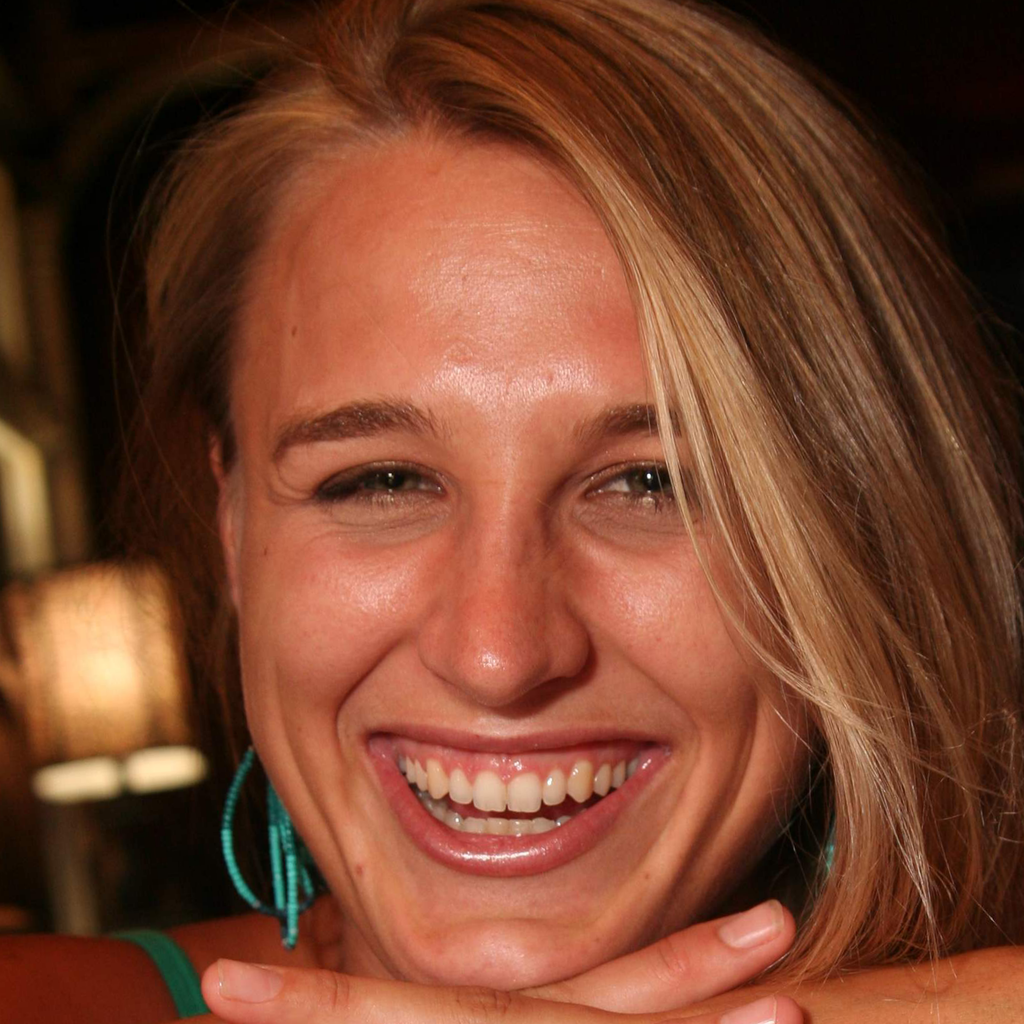
\includegraphics[height=1.6cm]{img/1.png}&
\hspace{1.3cm}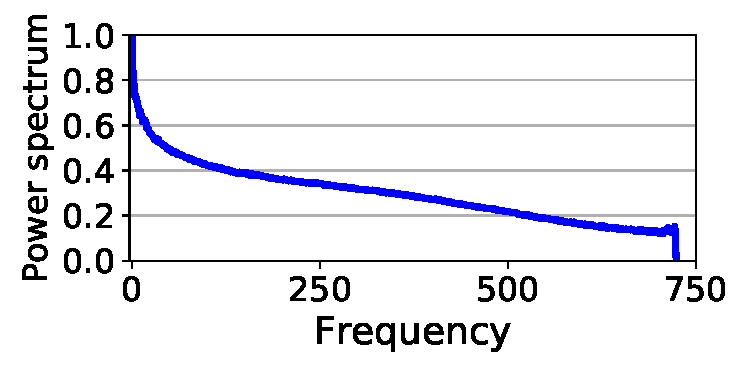
\includegraphics[height=1.8cm]{img/real_profiles_0.pdf}\\
%(a)\\
\hspace{0.9cm}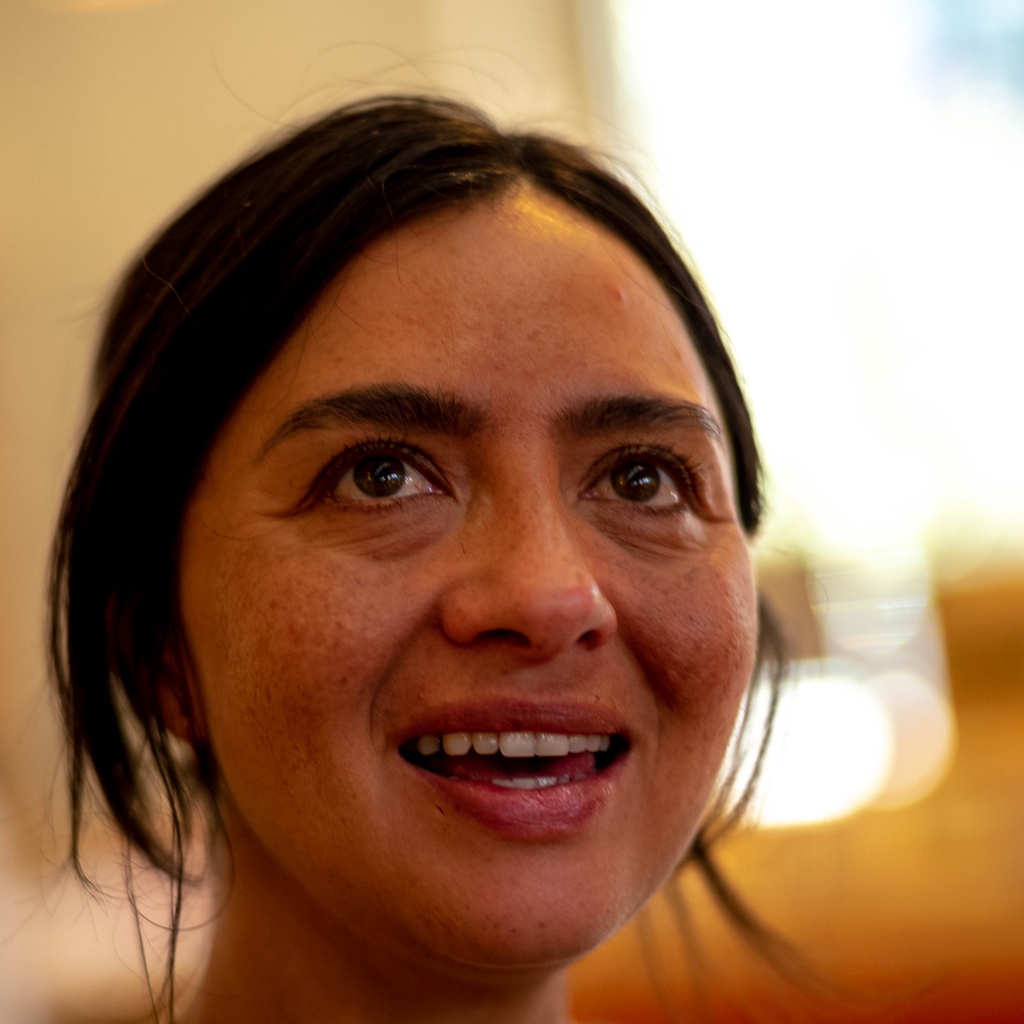
\includegraphics[height=1.6cm]{img/2.png}&
\hspace{1.3cm}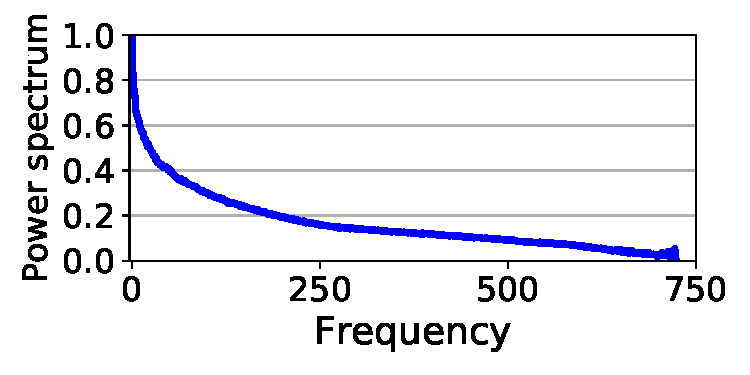
\includegraphics[height=1.8cm]{img/real_profiles_1.pdf}\\
%(b)\\
\hspace{0.9cm}
\includegraphics[height=1.6cm]{img/3.png}&
\hspace{1.3cm}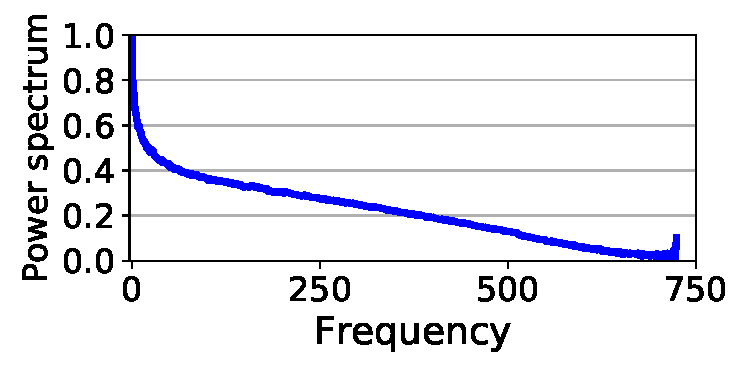
\includegraphics[height=1.8cm]{img/real_profiles_2.pdf}\\
%(c)
\end{tabular}
\end{minipage}
\hspace{0.5cm}
\begin{minipage}[t][][c]{1\columnwidth}
\centering
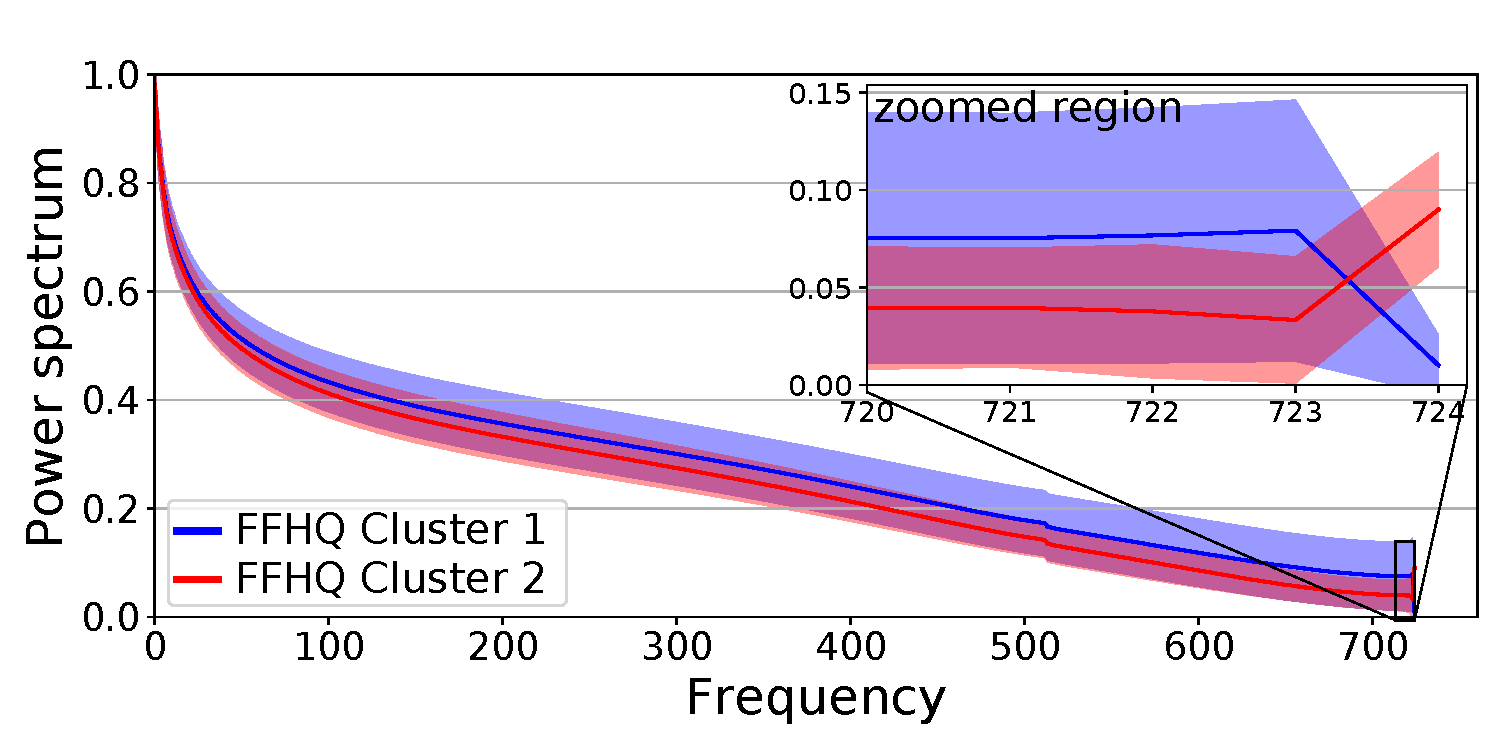
\includegraphics[width=1\textwidth]{img/ffhq_average4.pdf}
\end{minipage}
% \includegraphics[width=0.49\textwidth]{img/ffhq_average3.pdf}\\
 %(c)&(d)
  %  \end{tabular}
    \caption{(top) The frequency profiles from the FFHQ images are diverse, suggesting that their distribution is not uni-modal. (bottom) Average spectral profiles of the real data (FFHQ) after clustering with k-means (k=$2$). In the highest frequencies, the profiles can be well separated in two clusters.
    } 
    \label{fig1}
\end{figure}
% \iffalse
% \begin{figure*}[ht]
% \centering
% %\begin{tabular}{cc}
% \begin{minipage}[t][][b]{0.3\textwidth}
% \begin{tabular}{@{}c@{}c@{}}
% 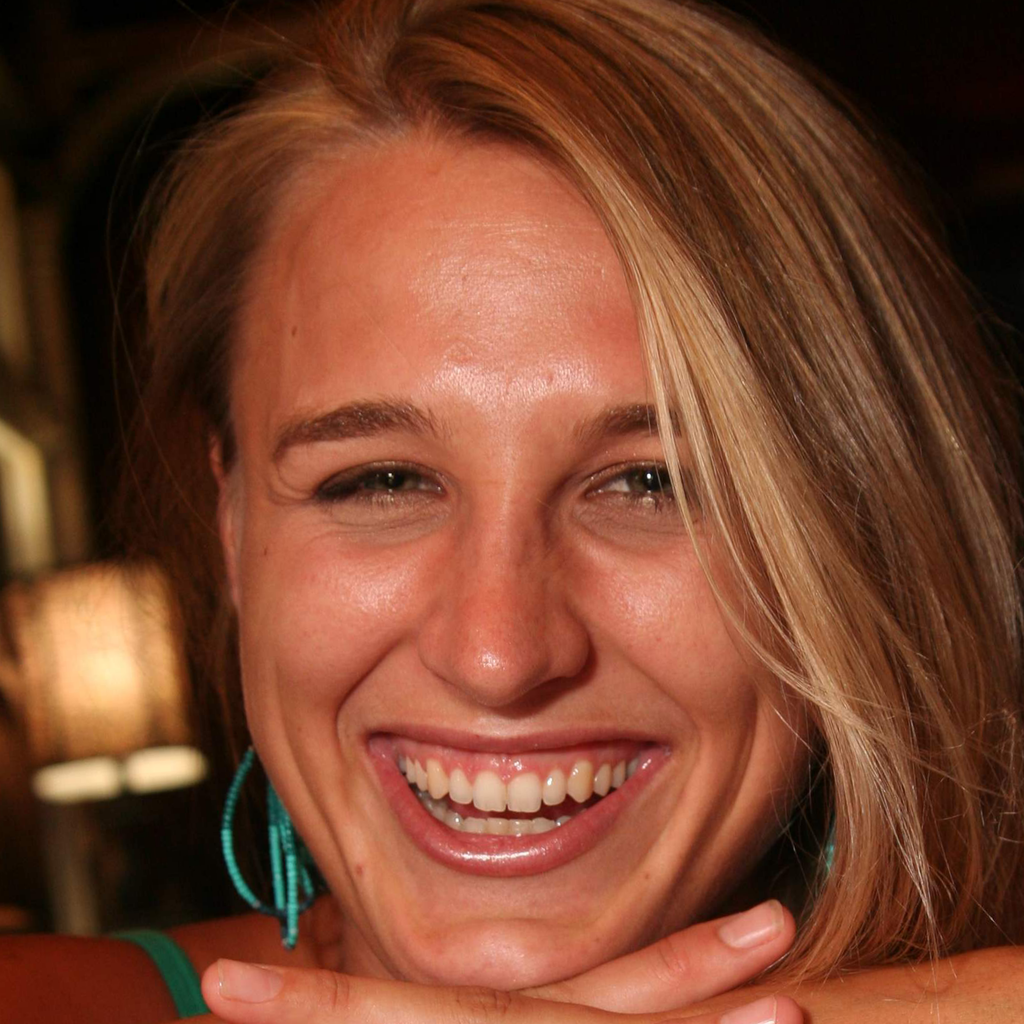
\includegraphics[height=1.6cm]{img/1.png}&
% 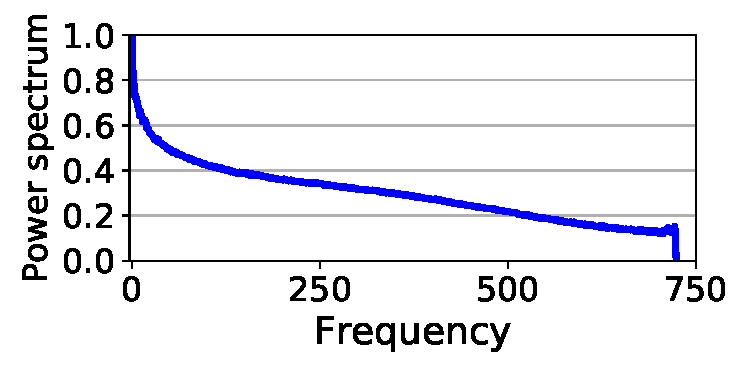
\includegraphics[height=1.8cm]{img/real_profiles_0.pdf}\\
% %(a)\\
% 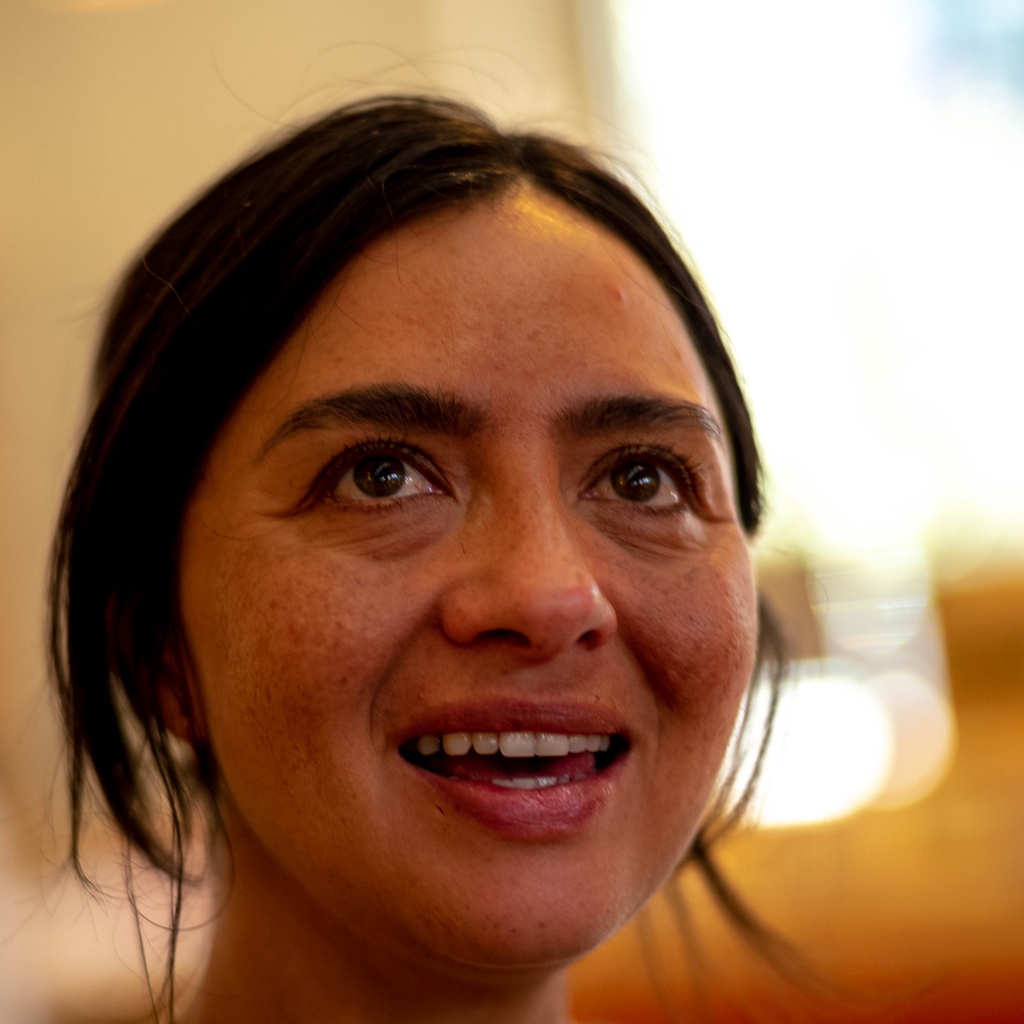
\includegraphics[height=1.6cm]{img/2.png}&
% 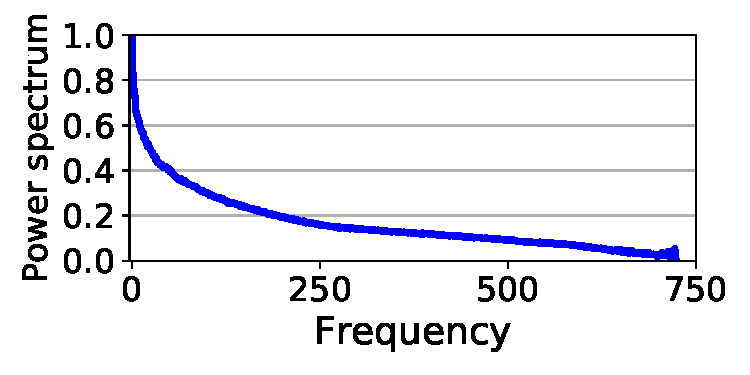
\includegraphics[height=1.8cm]{img/real_profiles_1.pdf}\\
% %(b)\\
% 
\includegraphics[height=1.6cm]{img/3.png}&
% 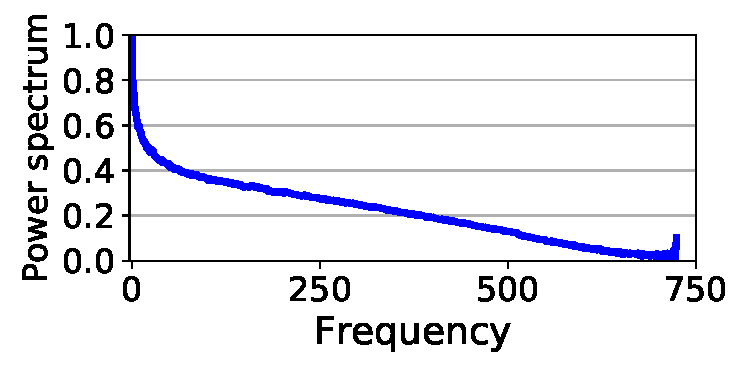
\includegraphics[height=1.8cm]{img/real_profiles_2.pdf}\\
% %(c)
% \end{tabular}
% \end{minipage}
% \hspace{0.5cm}
% \begin{minipage}[t][][c]{0.66\textwidth}
% \centering
% \includegraphics[width=0.95\textwidth]{img/ffhq_average3.pdf}
% \end{minipage}
% % \includegraphics[width=0.49\textwidth]{img/ffhq_average3.pdf}\\
%  %(c)&(d)
%   %  \end{tabular}
%     \caption{(top) The frequency profiles from the FFHQ images are diverse, suggesting that their distribution is not uni-modal. (bottom) Average spectral profiles of the real data (FFHQ) after clustering with k-means (k=$2$). In the highest frequencies, the profiles can be well separated in two clusters.
%     } 
%     \label{fig1}
% \end{figure*}\fi
which transforms a 2D image into a 2D array of its spatial frequencies. During up-sampling, an images frequency spectrum is altered depending on the up-sampling method. While bilinear interpolation results in smooth images with few high frequency components, the more commonly used "bed of nails" interpolation up-sampling, which fills the missing values with zeros, initializes the up-sampled image (or feature map) with many high frequency components. In \cite{margret2020upconvolution}, a theoretic analysis of the effect of upsampling using bed of nails interpolation is provided, which we summarize below.
\subsection{Spectral Effects of Up-Sampling.}
%Formulas similar to the CVPR paper by Ricard (I can copy those, but they will need reformating to single column. Please rephrase)
For simplicity,  \cite{margret2020upconvolution} consider in their analysis the case of one-dimensional signals, which generalizes to higher dimensions. For a signal $a$ the discrete Fourier Transform $\hat{a}$ is given by
\begin{equation}
\hat{a}_k=\sum_{j=0}^{N-1}e^{-2\pi i\cdot\frac{jk}{N}}\cdot a_j, \quad \mathrm{for }\quad k=0,\dots,N-1.
\end{equation}
Increasing $a$'s spatial resolution by factor $2$ results in %using a "bed of nails" interpolation
\begin{align}
\hat{a}^{up}_{\bar{k}}&=\sum_{j=0}^{2\cdot N-1}e^{-2\pi i\cdot\frac{j\bar{k}}{2\cdot N}}\cdot a^{up}_j
\nonumber\\
&=\sum_{j=0}^{N-1}e^{-2\pi i\cdot\frac{2\cdot j\bar{k}}{2\cdot N}}\cdot a_j
+ \sum_{j=0}^{N-1}e^{-2\pi i\cdot\frac{2\cdot (j+1)\bar{k}}{2\cdot N}}\cdot b_j,
\label{eq:theory2}
\end{align}
for $\bar{k}=0,\dots,2N-1$, where $b_j=0$ for "bed of nails" interpolation (and $b_j=a_j$ for nearest neighbor interpolation).
The first term in Eq. \eqref{eq:theory2} is similar to the original Fourier Transform while the second term is zero for $b_j=0$.  %, yet with the parameter $k$ being replaced by $\bar{k}$. Thus, 
It can be seen that if the spatial resolution is increased by a factor of $2$ the frequency axes are scaled by a factor of $\frac{1}{2}$. From sampling theoretic considerations, it is \cite{margret2020upconvolution}
\begin{align}
\eqref{eq:theory2}%hat{a}^{up}_\bar{k}&=\sum_{j=0}^{2\cdot N-1}e^{-2\pi i\cdot\frac{j\bar{k}}{2\cdot N}}\cdot a^{up}_j\\
&=\sum_{j=0}^{2\cdot N-1}e^{-2\pi i\cdot\frac{j\bar{k}}{2\cdot N}}\cdot \sum_{t=-\infty}^{\infty}a^{up}_j\cdot\delta(j-2t).\label{eq:theory3}
\end{align}

\iffalse
\begin{figure}[t]
   \begin{tabular}{ccc}
   &&&\\
   image $I$&magnitude of $\hat{I}$&spectral profile
   \end{tabular}
    \caption{Overview of the computation of the frequency profile. For an image $I$, the magnitude of its Fourier transform $\hat{I}$ contains the information of occurrences for each spatial frequency. The integral along the radii provides a 1D aggregation of this information.}
     \label{fig:azi}
\end{figure}
\fi


The point-wise multiplication with the Dirac impulse comb removes exactly the values for which $a^{up}=0$. In order to apply the convolution theorem~\cite{conv-theorem}, one has to assume $a$ being a periodic signal. Then, it is 
\begin{align}\hat{a}^{up}_{\bar{k}} &
%\eqref{eq:theory3}&
=\frac{1}{2}\cdot  \sum_{t=-\infty}^{\infty} \left(\sum_{j=-\infty}^{\infty}%{j=0}^{2\cdot N-1}
e^{-2\pi i\cdot\frac{j\bar{k}}{2\cdot N}}a^{up}_j\right)\left(\bar{k}-\frac{t}{2}\right)\, \nonumber\\
&\overset{\eqref{eq:theory2}}{=}\frac{1}{2}\cdot  \sum_{t=-\infty}^{\infty} \left(\sum_{j=-\infty}^{\infty}%{j=0}^{N-1}
e^{-2\pi i\cdot\frac{j\bar{k}}{N}}\cdot a_j\right)\left(\bar{k}-\frac{t}{2}\right).
\end{align}
Thus, the frequency spectrum $\hat{a}^{up}$ will contain replica of the frequency spectrum of $a$. More precisely, all frequencies beyond $\frac{N}{2}$ are up-sampling artifacts which can only be removed if the up-sampled signal is smoothed appropriately. 


In addition to these theoretic considerations \cite{margret2020upconvolution} also show practically that the correction of the resulting spectra is not possible with the commonly used $3\times 3$ convolutional filters.

%In the case of bilinear interpolation, we have $b_j=\frac{a_{j-1} + a_{j}}{2}$ in Eq.  \eqref{eq:theory2}, which corresponds to an average filtering of the values of $a$ adjacent to $b_j$. This is equivalent to a point-wise multiplication of $a^{up}$ spectrum $\hat{a}^{up}$ with a sinc function by their duality and the convolution theorem, which suppresses artificial high frequencies. Yet, the resulting spectrum is expected to be overly low in the high frequency domain.




%%%%%%%% 3 REAL DISTRIBUTION %%%%%%%%

\subsection{Analysis of Real Data Distribution}
\label{sec:distribution}
In order to analyze the distributions of the real as well as the generated images' frequency spectra, we consider an aggregate representation as done in \cite{margret2020upconvolution}. We compute the magnitude of the 2D spectral frequencies and integrate over the resulting 2D array for every radius to get a one-dimensional profile of the power spectrum, called \emph{azimuthal integral}
%the spatial frequencies $\omega_k$:
\begin{align}\label{eq:AI}
&AI(\omega_k)=  \int_0^{2\pi} \|\hat{I}\left(\omega_k\cdot \mathrm{cos}(\phi),\omega_k\cdot \mathrm{sin}(\phi)\right)\|^2 \mathrm{d}\phi\, \nonumber\\
&\mathrm{for }\quad k=0,\dots,M/2-1\, ,
\end{align}
assuming square images $I$. As pointed out in~\cite{margret2020upconvolution} this notation is obviously abusive for $\hat{I}$ being discrete. Practically, the integral is implemented as a sum over interpolated values. %\footnote{$\rightarrow M=N$. We are aware that this notation is abusive, since $\mathcal{F}(I)$ is discrete. However, fully correct discrete notation would only over complicated a side aspect of our work. A discrete implementations of AI is provided on \url{https://github.com/cc-hpc-itwm/UpConv}. }.
See Fig. \ref{fig1}(top) for some examples of real images from the Flickr-Faces-HQ dataset (FFHQ) \cite{karras2019StyleGAN} and their corresponding frequency profiles computed using Eq.~\eqref{eq:AI}. 

From these examples, one can see that the frequency profiles of the images are diverse and vary significantly, especially in the high frequency regime. Fig.~\ref{fig1}(bottom) shows the average frequency profiles after clustering the images of FFHQ by the magnitude of their highest frequency. The profiles can be well clustered into two groups just by looking at the highest frequency, which indicates that the frequency distribution of the real data can not be well approximated by a uni-modal Gaussian distribution as done in~\cite{margret2020upconvolution}. Since the true distribution is unknown, we argue that a suitable way of generating images with a higher spectral fidelity is to use an adversarial approach. Our model therefore contains an additional discriminator, taking as input the frequency profile of real and generated images.% (see section \ref{sec:model}).
\iffalse
\begin{figure}
\centering
 \includegraphics[width=\textwidth]{img/real_profiles.pdf}
    \includegraphics[width=0.8\textwidth]{img/ffhq_average2.pdf}
    \caption{(top) The frequency profiles from the FFHQ images are diverse, suggesting that their distribution is not uni-modal. (bottom) Clustered spectral profiles of real data (FFHQ) with k-means (k=$2$). In the highest frequencies, the profiles can be separated in two clusters.
    } 
    \label{fig1}
\end{figure}
\fi






%%%%%%%%%%%%%%%%%%%%%%%%%%%%%%%%%%%%%



%%%%%%%% 3 CLOAKING SCORE %%%%%%%%%%%

\subsection{GAN Evaluation in the Frequency Domain}
\label{sec:cloaking}
\begin{figure}[t]
    %\begin{subfigure}[t]{.5\textwidth}
        \centering
        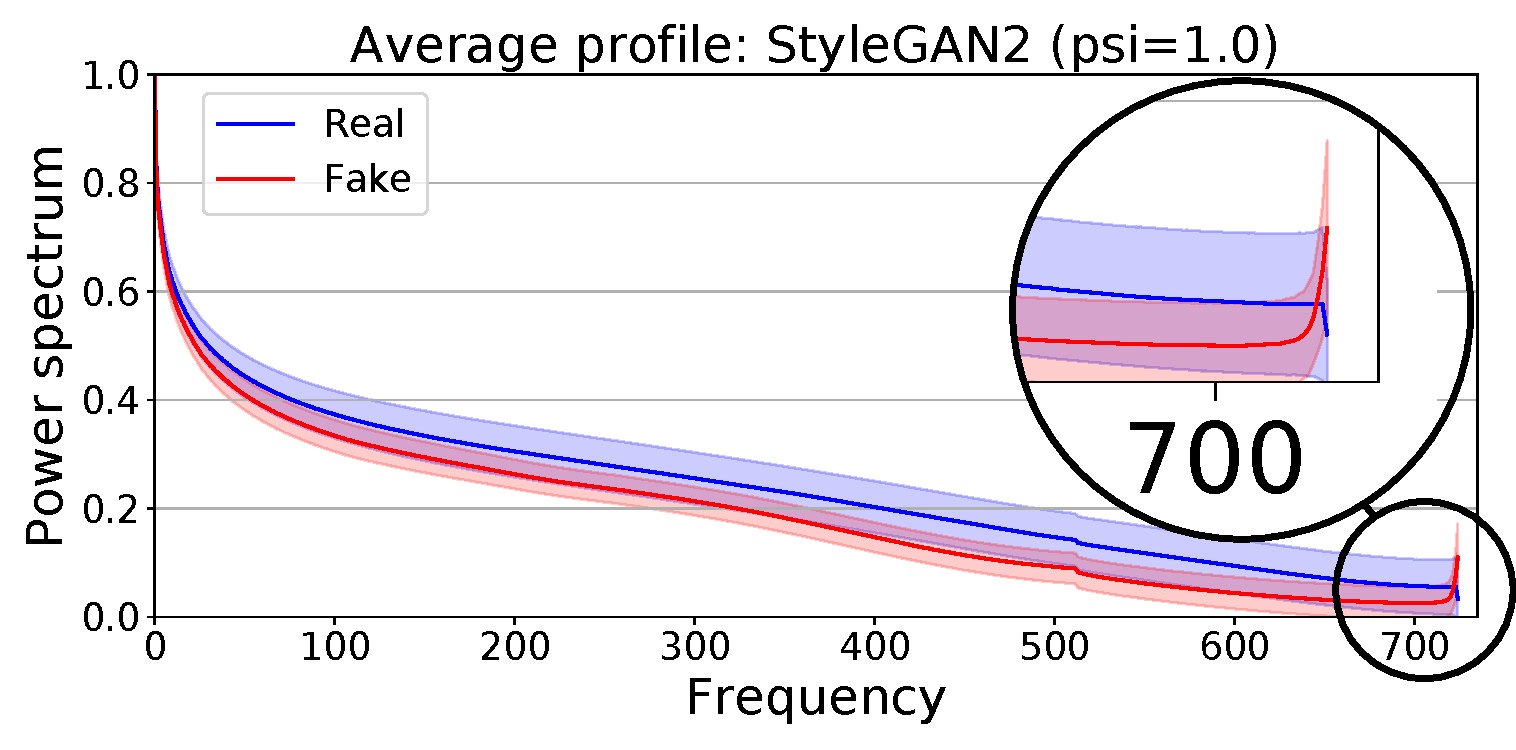
\includegraphics[width=\linewidth]{img/profiles.pdf}
        \caption{
            Average spectral profiles of real data (FFHQ) and data generated by StyleGAN2~\cite{karras2019StyleGAN2}.
            High frequency components in the generated images indicate grid artifacts or noise, which was not removed by the discriminator. 
%            It is obvious that spatially learning the real distribution is not sufficiently reflected in the frequency domain.
        }
        \label{fig:cprofiles}
    \end{figure}
    %\hfill
    \iffalse
    \begin{figure}[t]
        \centering
        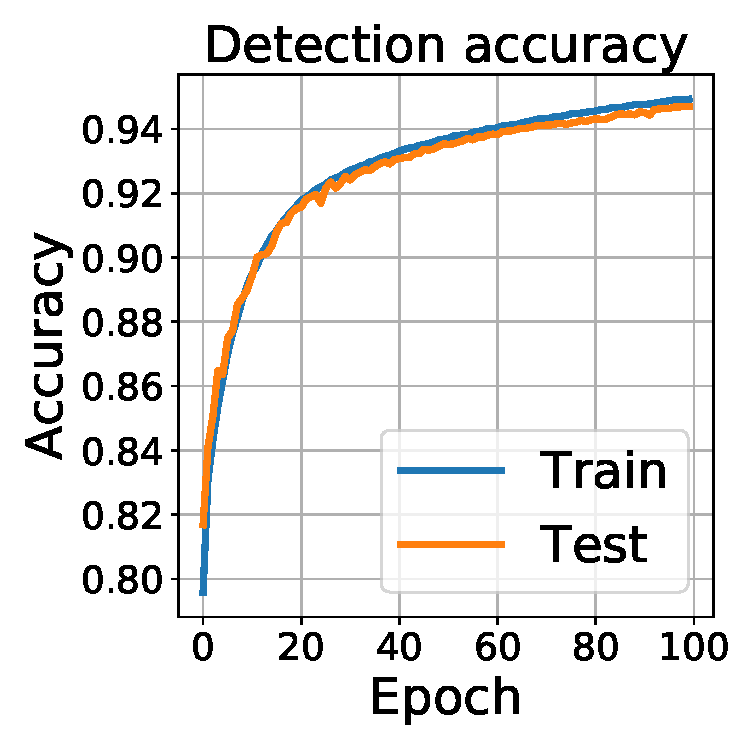
\includegraphics[width=0.6\linewidth]{img/detection_accuracy.pdf}
        \caption{
            Training and test accuracy of a Logistic Regression (LR) trained on $120k$ training images, $60k$ taken from FFHQ and $60k$ generated by StyleGAN2.
            $20k$ images are used for testing. The real and generated images can to a large degree be distinguished using LR.
        }
        \label{fig:cdetection}
    \end{figure}
    \fi
    %\caption{Average spectral profiles of FFHQ and StyleGAN2 and a Logistic Regression trained to separate both distributions.}
    %\label{fig:cloaking}
%\end{figure}
In general, the evaluation of the quality of generated images by GANs is highly subjective.
Therefore, \cite{heusel2017fid} introduced the \textit{Frchet Inception Distance} (FID) to provide a method of comparing different image generating models.
Since its proposal, this quality measure is widely adopted as one of the key indicators to proof the qualitative performance of GANs.
At the time of writing, StyleGAN2 \cite{karras2019StyleGAN2} is the best performing model according to FID, and trained on the FFHQ dataset.
Subjectively, generated images by StyleGAN2 are hard to distinguish from the real images.
This is reflected by a low FID score of $2.84 \pm 0.03$.
However, recent advances in DeepFake detection \cite{durall2019unmasking,margret2020upconvolution, frank2020leveraging} showed that it is possible to recognize such images using frequency domain representations.
Figure \ref{fig:cprofiles} shows the averaged profiles of a real data distribution, represented by FFHQ, and the corresponding images drawn from the learned distribution by StyleGAN2.
It is visible that the power spectrum is misaligned throughout most frequencies.
Images produced by StyleGAN2 contain high frequency components, which can be observed by a rapid increase in the power spectrum of the last frequencies. Such behavior indicates the presence of grid artifacts and high frequency noise. 
Thus, 
we argue that generated images should not only be assessed by their FID score but also by their spectral distribution fidelity and propose a method to evaluate the distribution alignment in the frequency domain, as a supplementary metric. %, supplementing the spatial measurements provided by FID.
Our method transforms images into spectral profile vectors by azimuthal integration (Eq.~\eqref{eq:AI}).
Then, we train a Logistic Regression on the spectral profiles given by all images taken from the real distribution, and a corresponding number of generated images given by a model. 
We then translate the training accuracy into a score according to %equation \eqref{eq:cloaking}.
\begin{equation}
    \text{Cloaking Score} = 1 - 2 \cdot \lvert \text{Accuracy} - 0.5 \rvert.
    \label{eq:cloaking}
\end{equation}

The \textit{Cloaking Score} (CS) ranges in $[0,1]$, where a score of $1.0$ indicates perfect spectral alignment, and a score of $0.0$ indicates that generated images can be linearly separated from real images in the spectral domain. For the StyleGAN2~\cite{karras2019StyleGAN2} example in Figure~\ref{fig:cprofiles}, the CS is 0.042 (acc. $0.979$) after $1\,000$ epochs, 0.022 (acc. $0.989$) after $10\,000$ epochs, and 0.018 (acc. $0.991$) after $40\,000$ training epochs.
%
%Figure \ref{fig:cdetection} shows the training progress of such a model.
%Training and testing accuracy are almost identical.
%Training accuracy increases progressively to $0.949$ after $100$ epochs, $0.979$ after $1\,000$ epochs, $0.989$ after $10\,000$ epochs, and $0.991$ after $40\,000$ epochs.
%We stopped training at this point.
%
Since the CS evaluation method gives rise to a trade-off between preciseness and runtime, we settled for scores after $1\,000$ epochs.
Runtime for $140k$ $64^2$-sized images is around $3$min, when all images are read from disk.


\iffalse
\begin{figure}
   \begin{tabular}{cc}
        %\centering
        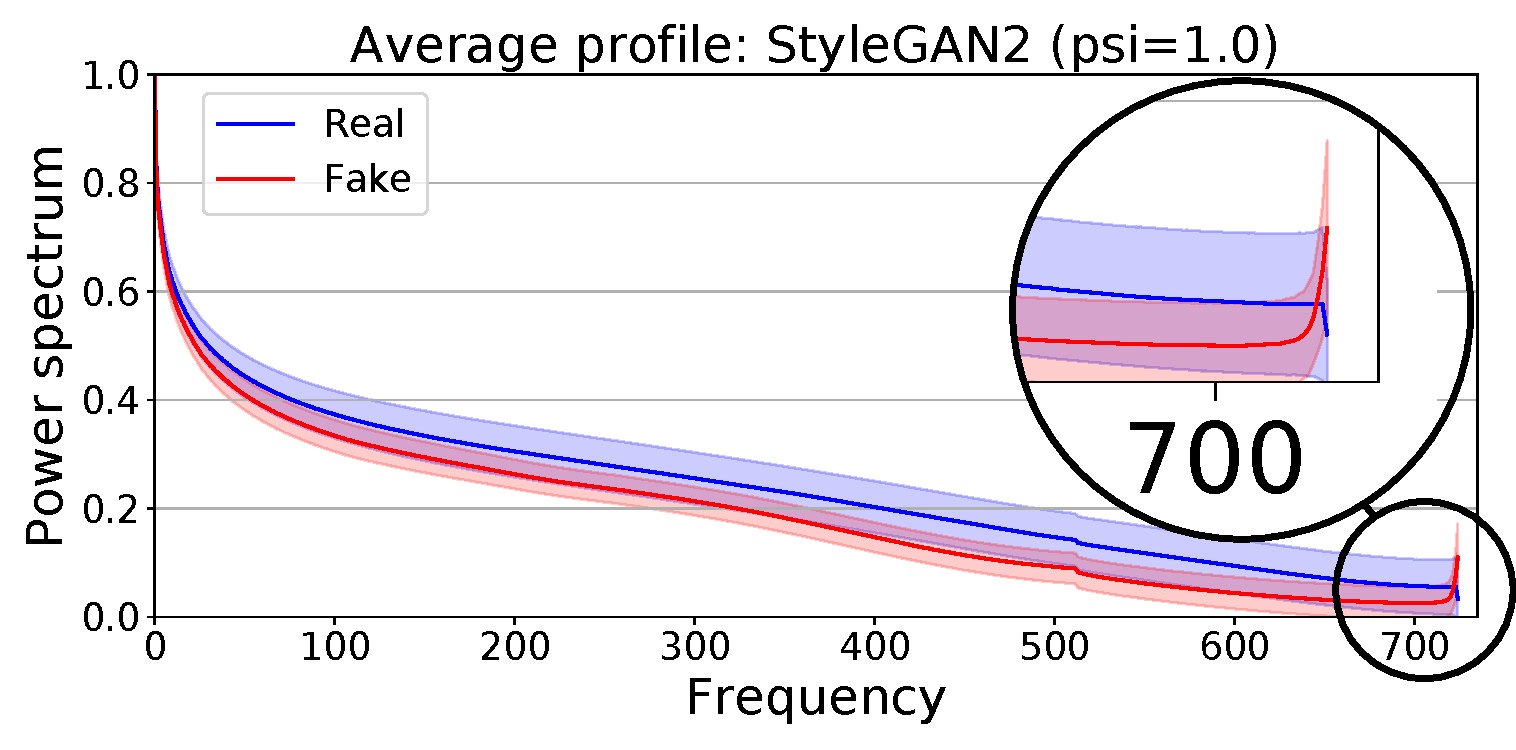
\includegraphics[width=0.63\linewidth]{img/profiles.pdf}&
       % \caption{
        %    Average spectral profiles of real data (FFHQ) and fake data (generated by StyleGAN2~\cite{karras2019StyleGAN2}).
         %   It is obvious that spatially learning the real distribution is not sufficiently reflected in the frequency domain.
        %}
     %   \label{fig:profiles}
    %
    %\hfill
    %\begin{subfigure}{.33\textwidth}
      %  \centering
        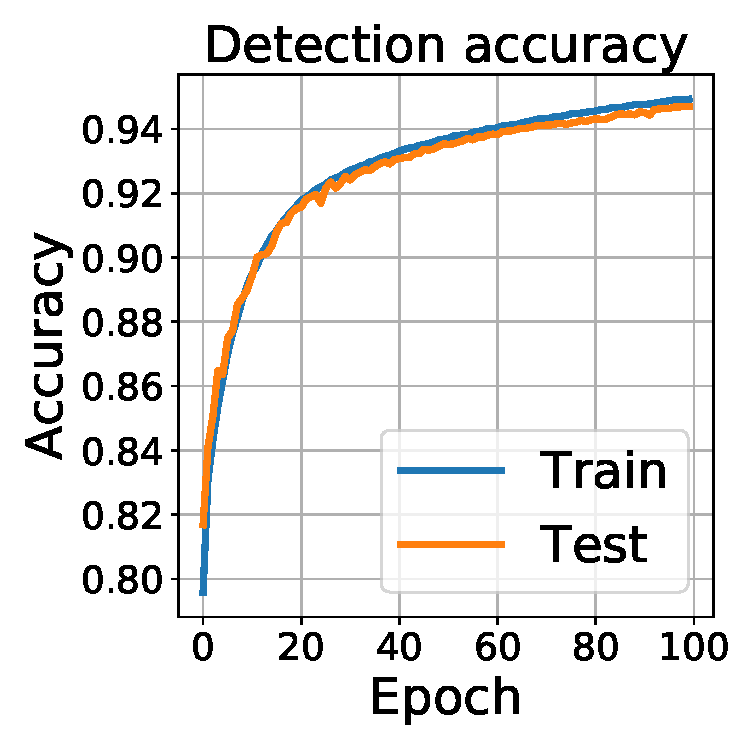
\includegraphics[width=0.34\linewidth]{img/detection_accuracy.pdf}\\
        Average spectral profiles of real data (FFHQ) and fake data (generated by StyleGAN2~\cite{karras2019StyleGAN2}).
            It is obvious that spatially learning the real distribution is not sufficiently reflected in the frequency domain.&
            Training and test accuracy of a Logistic Regression trained on $120k$ training images, $60k$ taken from FFHQ and $60k$ generated by StyleGAN2.
            $20k$ images are used for testing.
        \label{fig:detection}
    \end{tabular}
    \caption{Average spectral profiles of FFHQ and StyleGAN2 and a Logistic Regression trained to separate both distributions.}
    \label{fig:cloaking}
\end{figure}
\fi

%%%%%%%%%%%%%%%%%%%%%%%%%%%%%%%%%%%%%



%%%%%%%%%%%%%%%%%%%%%%% 4 MODEL %%%%%%%%%%%%%%%%%%%%%%%

\section{Learning to Generate Spectral Distributions}
\label{sec:model}
\begin{figure*}
\centering
    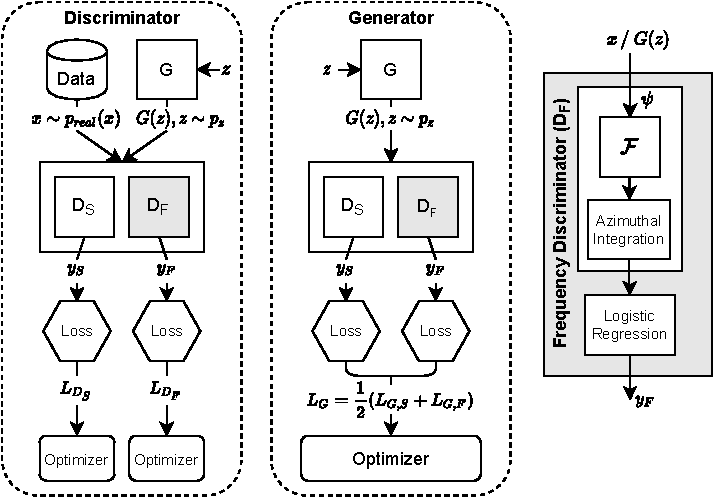
\includegraphics[width=0.75\textwidth]{img/Training-GCPR5.pdf}
    \caption{
    Training process of the proposed model.
    Losses are computed based on predictions representing the realness score of the given image in the spatial domain ($y_S$) as well as the frequency domain ($y_F$).
    Both spatial ($D_S$) and frequency ($D_F$) discriminators are trained separately by individual optimizer. % optimizer oder optimizers?
    When training generator $G$, both resulting losses are averaged.} 
    \label{fig:training}
\end{figure*}
Generative adversarial networks are trained in a minimax game between generator and discriminator networks, %where we optimize
%\begin{align}
%\min_G \max_D V(D,G)&=&\mathbb{E}_{{\bf x}\sim p_{\mathrm{data}}({\bf x})}[\mathrm{log}(D({\bf x})]\,+\,\quad\nonumber\\
%&&\mathbb{E}_{{\bf z}\sim p_{{\bf z}}({\bf z})}
%[\mathrm{log}\left(1-D(G({\bf z})\right)]\,
%\end{align}
where the discriminator wants to recognize generated images and the generator wants the discriminator to perform poorly, i.e.~to generate images which the discriminator can not tell apart from real ones, leading to objectives such as \cite{gan14nips}
\begin{align}
\min_G \max_D V(D,G)&=&\mathbb{E}_{{\bf x}\sim p_{\mathrm{data}}({\bf x})}[\mathrm{log}(D({\bf x}))]\,+\,\quad\nonumber\\
&&\mathbb{E}_{{\bf z}\sim p_{{\bf z}}({\bf z})}
[\mathrm{log}\left(1-D(G({\bf z}))\right)].\,
\end{align}
\citet{margret2020upconvolution} propose to add a penalty term, a \textit{Spectral Regularization}, to the generator to reduce discrepancies between the real and generated spectral distributions.
This regularization is implemented as a cross entropy loss on the $AI$ \eqref{eq:AI} profiles of the generator output, to minimize the difference of the generated images' spectra to the mean spectrum of real images.
% over a sample of real images, and comparing each generated image with this target profile.
%A penalty is added to the generator loss accounting for the extent of deviation from the mean average profile.
Hence, the generator tries to minimize this penalty by forcing each image to reflect the same, average profile.
In our experiments, this leads to an unstable training progress (see supplementary material). Out of $5$ runs, only $3$ models were able to reach $500$ epochs without degenerating due to mode collapse.
As we have shown above, the real spectral distribution is not a uni-modal Gaussian distribution around the average profile.
Instead, there are certain characteristics that the generator needs to be able to learn. The regularizer by \cite{margret2020upconvolution} seems suboptimal in this respect. Therefore, we argue that instead of learning one average profile, the generator should be taught to generate images according to the real data distribution in spatial as well as in spectral domain.

\begin{table}
    \caption{Investigated Discriminator Losses.}
    \label{tab0}
    \centering
    \begin{tabular}{ll}
    \toprule
    $\mathcal{L}_{\mathrm{DCGAN}}$& $- \mathbb{E}_{{\bf x}%\sim p_{\mathrm{d}}
    }
    [\mathrm{log}(D({\bf x}))]\,-\,
\mathbb{E}_{{\bf \hat{x}}%\sim p_{\mathrm{g}}
}
[\mathrm{log}\left(1-D({\bf \hat{x}})\right)]$\\
$\mathcal{L}_{\mathrm{LSGAN}}$& $- \mathbb{E}_{{\bf x}%\sim p_{\mathrm{d}}
}[(D({\bf x})-1)^2]\,+\,
\mathbb{E}_{{\bf \hat{x}}%\sim p_{\mathrm{g}}
}
[D({\bf \hat{x}})^2]$\\
$\mathcal{L}_{\mathrm{WGAN}}$& $- \mathbb{E}_{{\bf x}%\sim p_{\mathrm{d}}
}[D({\bf x})]\,+\,
\mathbb{E}_{{\bf \hat{x}}
%\sim p_{\mathrm{g}}
}
[D({\bf \hat{x}})]$\\
$\mathcal{L}_{\mathrm{WGAN-GP}}$& $\mathcal{L}_{\mathrm{WGAN}}+$\\
&$\lambda \mathbb{E}_{{\bf \hat{x}} %\sim p_{\mathrm{g}}
}[(\|\nabla D(\alpha {\bf x}+(1-\alpha {\bf \hat{x}}))\|_2-1)^2] $\\

    \bottomrule
    
    \end{tabular}
    \end{table}

%Therefore, we propose a different approach.
%Starting from a DCGAN \cite{radford2015dcgan} architecture, w
We propose to use a second discriminator network ($D_F$) for this purpose (see Figure \ref{fig:training}).
While one could obviously consider to use full 2D power spectra and a convolutional architecture as in the original discriminator, we argue that an additional discriminator should be as lightweight and modular as possible.
The proposed frequency spectrum discriminator $D_F$ takes as input real or generated images which then go through a spectral transformation layer $\psi$ that computes the magnitude of their Fourier transform.
%Then,
Afterwards, the azimuthal integral (Eq.~\eqref{eq:AI}) is computed, projecting the 2D spectrum onto a 1D vector. Then, we add a fully connected layer with Sigmoid activation function, which is trained to discriminate between real and generated images. 

Such a simple discriminator can in principle be trained with any of the commonly used GAN loss functions. To investigate the dependency of the discriminator performance on the employed loss, we consider models with the commonly used loss functions in Tab. \ref{tab0} and focus on simple architectures (i.e. DCGAN \cite{radford2015dcgan}, LSGAN \cite{mao2017least}, and Wasserstein GAN (WGAN)~\cite{gulrajani2017wgan,gulrajani2017improved}).
%In the case of DCGAN as baseline architecture, it is trained with binary cross entropy (BCE) loss, but we also investigate its performance in conjunction with d can be adapted to other losses for example in the case of Wasserstein GAN (WGAN)~\cite{gulrajani2017wgan,gulrajani2017improved} or Least Squares GAN (LSGAN)~\cite{mao2017least}. 

We train both the spatial ($D_S$) and the frequency ($D_F$) discriminators by separate losses, applying the same loss function (e.g.~BCE in case of DCGAN). For training the generator $G$, both resulting losses are combined by averaging (see Fig.~\ref{fig:training}). 
%This spectral discriminator is composed of a spectral transformation layer $\psi$ and a logistic regression, learning to distinguish between real and fake spectral profiles.
%
Additionally, we keep the proposed architectural suggestions by \cite{margret2020upconvolution}, namely increasing the last upconvolutional layer to $8 \times 8$, and adding an additional block of three $5 \times 5$ to the end of the generator network, which, as they argue empirically, is necessary to provide the network with the capacity to "repair" the spectral artifacts.  
%This spectral discriminator is composed of a spectral transformation layer $\psi$ and a logistic regression, learning to distinguish between real and fake spectral profiles.
%Layer $\psi$ implements the same functionality used in section \ref{sec:cloaking}
\paragraph{Implementation Details.}
The memory comsumption of the proposed discriminator depends on the image width and height $n$ and adds only  $\left\lceil n/\sqrt{2} \right\rceil + 1$ parameters. We evaluate it with different architectures.
% $\left\lceil \sqrt{2 \cdot (n/2)^2} \right\rceil + 1$
DCGAN, LSGAN and WGAN-GP were trained using Adam optimizer, for WGAN, we used RMSprop, with a learning rate of $0.0002$ and a batch size of $128$ for $500$ epochs. In all cases, we apply the same loss function on both discriminators.
% To finetune StyleGAN2 we use the standard settings provided by their implementation.


%%%%%%%%%%%%%%%%%%%%%%% 5 EXPERIMENTS %%%%%%%%%%%%%%%%%

\section{Experiments}
\label{sec:experiments}
\begin{table}
    \caption{Evaluation of the architectural change by \citet{margret2020upconvolution} on the image generation quality for DCGAN and LSGAN at $64^2$ pixel resolution. In both cases, the changed up-sampling and additional convolutional layers lead to an improved FID and spectral difference, while the cloaking score is low.}
    % \label{tab1}
    \centering
    \begin{tabular}{l c c c}
        \toprule
       % &&\multicolumn{2}{|c|}{transfer}&\multicolumn{1}{|c|}{}\\
         Model & FID $\downarrow$ & SD $\downarrow$ & CS $\uparrow$ \\
        \midrule
DCGAN$_{orig}$ & 17.749 & 1.510 & {\bf 0.35} \\
DCGAN &{\bf 15.257} &{\bf 1.293} & 0.16\\
LSGAN$_{orig}$&18.423&1.602&{\bf 0.28}\\
LSGAN& {\bf 15.518} & {\bf 0.468} & 0.04\\
\bottomrule
    \end{tabular}
    \label{tab:taborig}
\end{table}

\begin{table*}
    %\caption{(left) FID, Spectral Difference (SD) and Cloaking Score (CS) of the original models and models with the proposed discriminator. %In all cases, the spectral distribution can be fit without increasing the FID. 
    %(right) The detection accuracies of recent methods by \citet{margret2020upconvolution} and \citet{Wang_2020_CVPR} (Durall et al.$^*$ are trained on the original GAN model and tested on the models with regularized/corrected power spectra.).} %With our discriminator, the detection of generated images becomes significantly harder for the frequency based approach from \citet{margret2020upconvolution}. }
    \caption{Evaluation of the proposed discriminator in terms of GAN quality measures and generated image detection scores. %While the FID is not affected, the cloaking score is increased and detector quality decreases when our model is applied.
    }
    \label{tab1}
    %\resizebox{1\textwidth}{!}
    %{
    \small
    \centering
    \begin{tabular}{l|l|ccc|ccccc}
        \toprule
        &&\multicolumn{3}{c}{GAN Quality}&\multicolumn{5}{c}{Detection Accuracy}\\
         &&&&&\multicolumn{2}{c}{Durall et al.$^*$}
        &\multicolumn{2}{c}{Durall et al.}&Wang et al.\\
        Size & Model & FID $\downarrow$ & SD $\downarrow$ & CS $\uparrow$ & SVM $\downarrow$ & LR $\downarrow$ & SVM $\downarrow$ & LR $\downarrow$ & ACC $\downarrow$ \\
        %Size & Model & FID & SD  & CS \\
        \midrule
    %     DCGAN    &  25.6    &  0.21 \\
    %     DCGAN + \cite{margret2020upconvolution}     & 37.3 & 0.19 \\
    %   %  \hline
    %     DCGAN, Spectral    &  \textbf{24.0}   &  \textbf{0.63} \\
    %     \hline
    %     LSGAN    &  39.0    &  0.01 \\
    %     LSGAN, Spectral    &  33.6    &  0.61 \\
    %     \hline
    %     WGAN    &  33.8    &  0.14 \\
    %     WGAN, Spectral    &  35.7    &  0.01 \\
    %     \hline
\multicolumn{1}{c|}{\multirow{9}{*}{$64^2$}} 
& DCGAN & {\bf 15.257} & 1.293 & 0.16& 0.89&0.89& 0.89&0.89  &0.81\\
& DCGAN (Durall et al.)& 29.875 & 0.311 & 0.25 & 0.51&{\bf 0.49}& 0.79&0.82&0.67 \\
 & DCGAN, Spectral & 15.591 & {\bf 0.042} & {\bf 0.84}  &{\bf 0.50} &0.50 &{\bf 0.59}&{\bf 0.58}&{\bf 0.66}\\ %\cline{2-5}
 & LSGAN & 15.518 & 0.468 & 0.04 & 0.94 & 0.94& 0.94 & 0.94&0.67\\
 & LSGAN, Spectral & {\bf 15.515} & {\bf 0.041} & {\bf 0.86}  & {\bf 0.51} & {\bf 0.50} & {\bf 0.55}&{\bf 0.56}&{\bf 0.64}\\ %\cline{2-5}
 & WGAN & {\bf 47.704} & 1.291 & 0.01 & 0.99&0.99&0.99&0.99&0.79\\
 & WGAN, Spectral & 47.948 & {\bf 0.029} & {\bf 0.85} & {\bf 0.50}&{\bf 0.50} & {\bf 0.62}&{\bf 0.65}&0.79\\ %\cline{2-5}
 & WGAN-GP & {\bf 39.404} & 0.575 & 0.18 & 0.92&0.94&0.92&0.94&0.76\\
 & WGAN-GP, Spectral & 39.441 & {\bf 0.252} & {\bf 0.54} &{\bf 0.51}&{\bf 0.51}&{\bf 0.75}&{\bf 0.76}&{\bf 0.65}\\ \midrule
\multicolumn{1}{c|}{\multirow{9}{*}{$128^2$}} & DCGAN & 19.908 & 1.579 & 0.00  & 0.99 & 0.99 &0.99&0.99 &0.82\\
& DCGAN (Durall et al.) & 41.896 & 0.449 & 0.08 & \bf{0.51} & 0.51 & 0.98 & 0.98 & 0.87\\
 & DCGAN, Spectral & {\bf 19.898} & {\bf 0.087} & {\bf 0.72} & {\bf 0.51}&{\bf 0.50}&{\bf 0.66}&{\bf 0.69}&{\bf 0.81} \\ %\cline{2-5}
 & LSGAN & 20.850 & 3.786 & 0.01  & 0.99 &0.99&0.99&0.99&0.81\\
 & LSGAN, Spectral & {\bf 19.043} & {\bf 0.074} & {\bf 0.76} &  {\bf 0.50}& {\bf 0.50} & {\bf 0.82}&{\bf 0.83}&{\bf 0.80}\\ %\cline{2-5}
 & WGAN & {\bf 20.757} & 1.996 & 0.01& 0.99 & 0.99 & 0.99&0.99 &0.83 \\
 & WGAN, Spectral & 24.568 & {\bf 0.136} & {\bf 0.66} & {\bf 0.52}& {\bf 0.53} &{\bf 0.61} &{\bf 0.60}&{\bf 0.81}\\ %\cline{2-5}
 & WGAN-GP & 47.630 & 2.349 & 0.02 &  0.99& 0.99 &   0.99& 0.99&0.96\\ 
 & WGAN-GP, Spectral & {\bf 42.740} & {\bf 0.260} & {\bf 0.38}  &  {\bf 0.50}&{\bf 0.50}& {\bf 0.82} & {\bf 0.83}&{\bf 0.62} \\\midrule
\multicolumn{1}{c|}{\multirow{5}{*}{$256^2$}} & DCGAN & {\bf 20.132} & 9.826 & 0.00 & 1.00 & 1.00 & 1.00 & 1.00 & 0.96\\
 & DCGAN (Durall et al.) & 29.813 & 0.786 & 0.01 & 0.50 & 0.50 & 1.00 & 0.99 & 0.99 \\
 & DCGAN, Spectral & 20.863 & {\bf 0.229} & {\bf 0.50}&{\bf 0.50}& {\bf 0.50} &  {\bf 0.89}&{\bf 0.93}&{\bf 0.85} \\ %\cline{2-5}
 & LSGAN & 19.893 & 5.955 & 0.00 & 1.00 & 1.00 & 1.00 & 1.00 & 0.85\\
 & LSGAN, Spectral & {\bf 19.884} & {\bf 0.216} & {\bf 0.46}  &{\bf 0.50} &{\bf 0.50}  & {\bf 0.77}&{\bf 0.82}&{\bf 0.72}\\
% & WGAN & 29.294 & 1.653 & 0.01 \\
% & WGAN, Spectral & 244.296 & 0.659 & 0.16 \\ \cline{2-5}
% & WGAN-GP & 42.141 & 9.357 & 0.00 \\
% & WGAN-GP, Spectral & 45.899 & 1.039 & 0.01 \\ \hline
\bottomrule

% \midrule
% \multicolumn{1}{c|}{\multirow{2}{*}{$1024^2$}} & StyleGAN2 & {\bf 2.733} & 32.250 & 0.09 &  & & & & 0.76 \\
% & StyleGAN2, Spectral & 3.326 & {\bf 5.978} & {\bf 0.24} & & & & &\\

% ungenderte Architektur
% 64 & DCGAN & 17.749 & 1.510 & 0.35 \\
% 64 & LSGAN & 18.423 & 1.602 & 0.28 \\
% 64 & DCGAN, Spectral & 17.218 & 0.075 & 0.80 \\
% 64 & LSGAN, Spectral & 18.734 & 0.036 & 0.87 \\
%\vspace{-0.5cm}
    \end{tabular}
%}
\end{table*}

\begin{table}
    \caption{Evaluation of the finetuned StyleGAN2.}
    \label{tab1-stylegan}
    \small
    \centering
    \begin{tabular}{l|l|ccc}
        \toprule
        &&\multicolumn{3}{c}{GAN Quality}\\
        Size & Model & FID $\downarrow$ & SD $\downarrow$ & CS $\uparrow$ \\
        \midrule
            \multicolumn{1}{c|}{\multirow{2}{*}{$1024^2$}} & StyleGAN2 & {\bf 2.733} & 32.250 & 0.09 \\
            & StyleGAN2, Spectral & 3.326 & {\bf 5.978} & {\bf 0.24} \\
        \bottomrule
    \end{tabular}
        
\end{table}

\iffalse
\begin{table}
    \caption{Detection Scores by \cite{margret2020upconvolution}}
    % \label{tab1}
    \centering
    \begin{tabular}{l|l|rr|rr}
        \toprule
        &&\multicolumn{2}{c|}{transfer}&\multicolumn{2}{c}{}\\
        Size & Model &SVM&LR&SVM&LR \\
        \midrule
\multicolumn{1}{c|}{\multirow{8}{*}{$64^2$}} 
& DCGAN & 0.89&0.89& 0.89&0.89\\
& DCGAN baseline & 0.51&0.49& 0.79&0.82\\
 & DCGAN, Spectral &0.50 &0.50 &0.59&0.58\\ 
 %& DCGAN & 0.85&0.837&0.85&0.84 \\
%& DCGAN baseline & 0.52&0.51&0.73&0.72\\
% & DCGAN, Spectral &0.49 &0.48 &0.57&0.57\\ 
 \cline{2-6}
 & LSGAN & 0.94 & 0.94& 0.94 & 0.94\\
 & LSGAN, Spectral & 0.51 & 0.50 & 0.55&0.56 \\ \cline{2-6}
 & WGAN & 0.99&0.99&0.99&0.99\\
 & WGAN, Spectral & 0.50&0.50 & 0.62&0.65 \\ \cline{2-6}
 & WGAN-GP & 0.92&0.94&0.92&0.94 \\
 & WGAN-GP, Spectral&0.51&0.51&0.75&0.76\\ \midrule
\multicolumn{1}{c|}{\multirow{8}{*}{$128^2$}} & DCGAN & 0.99 & 0.99 &0.99&0.99 \\
 & DCGAN, Spectral & 0.51&0.50&0.66&0.69 \\ \cline{2-6}
 & LSGAN & 0.99 &0.90&0.99&0.99  \\
 & LSGAN, Spectral &  0.50& 0.50 & 0.82&0.83  \\ \cline{2-6}
 & WGAN & 0.99 & 0.99 & 0.99&0.99 \\
 & WGAN, Spectral & 0.52& 0.53 &0.61 &0.60 \\ \cline{2-6}
 & WGAN-GP &  0.99& 0.99 &   0.99& 0.99 \\ 
 & WGAN-GP, Spectral &  0.50&0.50& 0.82 & 0.83 \\\midrule
\multicolumn{1}{c|}{\multirow{4}{*}{$256^2$}} & DCGAN & 1.0&1.0&1.0&1.0  \\
 & DCGAN, Spectral &  0.5& 0.5 &  0.89&0.93\\ \cline{2-6}
 & LSGAN & 1.0 & 1.0 & 1.0&1.0 \\
 & LSGAN, Spectral &0.5 &0.5  & 0.77&0.82\\ \bottomrule
% & WGAN & 29.294 & 1.653 & 0.01 \\
% & WGAN, Spectral & 244.296 & 0.659 & 0.16 \\ \cline{2-5}
% & WGAN-GP & 42.141 & 9.357 & 0.00 \\
% & WGAN-GP, Spectral & 45.899 & 1.039 & 0.01 \\ \hline
    \end{tabular}
  
\end{table}

\begin{table}
    \caption{Detection Scores by Wang et al. (CVPR 20)}
    % \label{tab1}
    \centering
    \begin{tabular}{l|l|rr}
        \toprule
       % &&\multicolumn{2}{|c|}{transfer}&\multicolumn{1}{|c|}{}\\
        Size & Model & AP&ACC\\
        \midrule
        
\multicolumn{1}{c|}{\multirow{8}{*}{$64^2$}} 
& DCGAN & 89.60&80.81 \\
& DCGAN baseline &78.28&67.09\\
% & DCGAN, Spectral &80.17&68.81\\ 
  & DCGAN, Spectral &77.09&66.35\\ 
 %& DCGAN & 0.85&0.837&0.85&0.84 \\
%& DCGAN baseline & 0.52&0.51&0.73&0.72\\
% & DCGAN, Spectral &0.49 &0.48 &0.57&0.57\\ 
 \cline{2-4}
 & LSGAN &68.61&67.31 \\
 & LSGAN, Spectral &74.29&63.58 \\ %\cline{2-4}
 & WGAN & 88.40&78.95\\
 & WGAN, Spectral &  89.11&79.45\\ \cline{2-4}
 & WGAN-GP & 86.07&75.58\\
 & WGAN-GP, Spectral&77.02&65.05\\ \midrule
\multicolumn{1}{c|}{\multirow{8}{*}{$128^2$}} & DCGAN &96.67&81.73\\
 & DCGAN, Spectral & 96.39&80.8\\ \cline{2-4}
 & LSGAN & 96.43&80.53 \\
 & LSGAN, Spectral &96.1&79.7  \\ \cline{2-4}
 & WGAN &96.97&82.93  \\
 & WGAN, Spectral& 96.56&81.20\\ \cline{2-4}
 & WGAN-GP &99.49&95.55  \\ 
 & WGAN-GP, Spectral &86.65&62.44 \\\midrule
\multicolumn{1}{c|}{\multirow{4}{*}{$256^2$}} & DCGAN &99.93& 96.11\\
 & DCGAN, Spectral &99.61&84.79\\ \cline{2-4}
 & LSGAN & 99.53&85.19 \\
 & LSGAN, Spectral &  \\ \bottomrule
% & WGAN &  \\
% & WGAN, Spectral &  \\ \cline{2-5}
% & WGAN-GP & \\
% & WGAN-GP, Spectral &  \\ \hline

    \end{tabular}
\end{table}
\fi

% change in runtime?
% FID/Spectral loss rolling average (last 5 epochs?)
% plot: wie unseres ber epochen fittet
% plot: ricard vs uns spektren

% Measurements conducted during training: FID/SL on 10k generated images after each epoch.
% Experiments are conducted on the Flickr-Faces-HQ (FFHQ) dataset \cite{karras2019style}, which contains $70$~$000$ high-quality face images at $1024 \times 1024$ resolution, which show large variations in terms of age and ethnicity and have diverse backgrounds.
Experiments are conducted on the FFHQ dataset, which contains $70$~$000$ high-quality face images at $1024 \times 1024$ resolution showing large variations in terms of age, ethnicity, and backgrounds.
From this dataset, we downsample three versions in resolution $64\times64$, $128\times128$ and $256\times256$.
We evaluate all experiments on 10k examples in terms of FID and the proposed cloaking score (CS). If the distribution of the real data is matched in both spatial and frequency domain, the resulting FID should be low while the cloaking score should be high. Additionally, we report the sum of absolute differences between the average profile of 10k generated images with the average profile of all real images, denoted as \textit{spectral difference} (SD).
This measure is similar to the optimization target in~\cite{margret2020upconvolution}.

First, we validate the impact of adding additional convolutional layers and increasing the filter size to $5\times5$ as suggested by \citet{margret2020upconvolution} on DCGAN and LSGAN (see Tab.~\ref{tab:taborig}).
In both cases, the modification leads to an improved FID and a lower spectral difference. Yet, the cloaking score is even lower than the one of the baseline approach, indicating that the generated distributions are still linearly separable from their integrated frequency spectra ($AI$, Eq.~\eqref{eq:AI}). This leads to two observations: (1) Increasing the amount of convolutions at the highest resolution can increase image quality of simple GAN methods, and (2) the conventional spatial discriminator does not provide the necessary signal to bring the spectral distributions closer together.
From these observations, we continue with the modified networks to investigate whether the proposed spectral discriminator can provide the necessary training signal, and is able to use the network capacity, to assimilate the generated images' frequency spectra to the real distribution.

To evaluate the proposed spectral discriminator $D_F$ in the context of diverse losses, we train variants of \mbox{DCGAN} \cite{radford2015dcgan}, LSGAN~\cite{mao2017least}, WGAN~\cite{arjovsky2017wasserstein} and WGAN~GP~\cite{gulrajani2017improved} with and without $D_F$.
%
 While the modified DCGAN and LSGAN models can generate images at up to $256^2$ pixel resolution, the training behavior of the Wasserstein GANs becomes easily unstable. Thus, we only consider them until $128^2$ pixels resolution.
Additionally, to evaluate scalability to high resolutions, we finetune a pretrained state-of-the-art model, StyleGAN2, after adding $D_F$ to its training process.

\begin{figure}
    \begin{subfigure}[t]{.49\columnwidth}
        \centering
        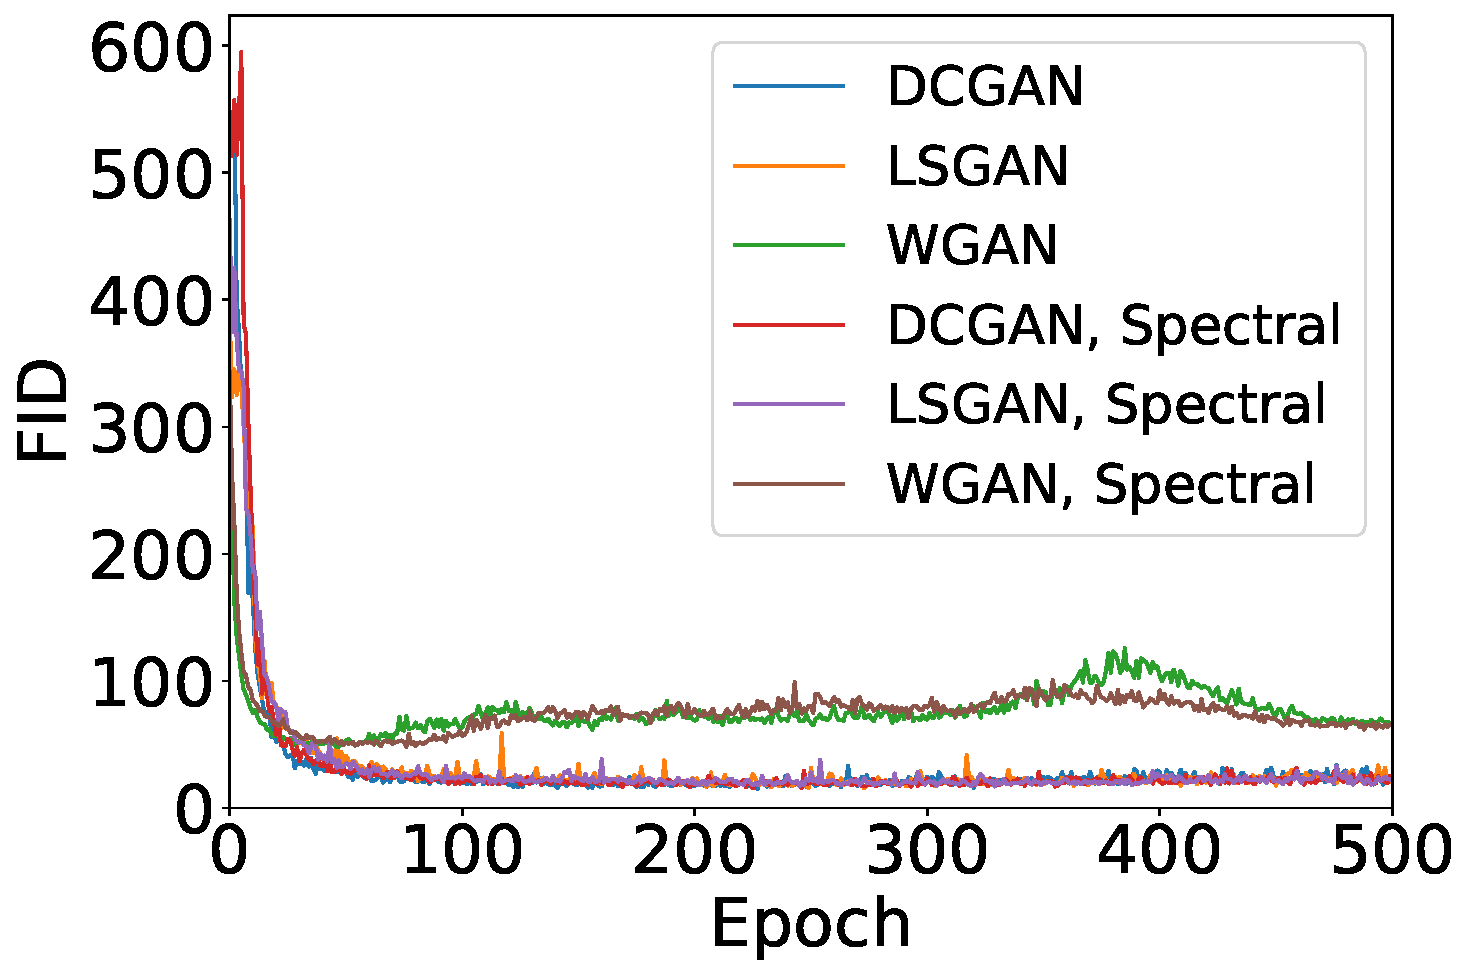
\includegraphics[width=\linewidth]{img/training_fid.pdf}
        \caption{
            The resulting FID scores are similar, and the training is stable.
        }
        \label{fig:profiles}
    \end{subfigure}
    \hfill
    \begin{subfigure}[t]{.49\columnwidth}
        \centering
        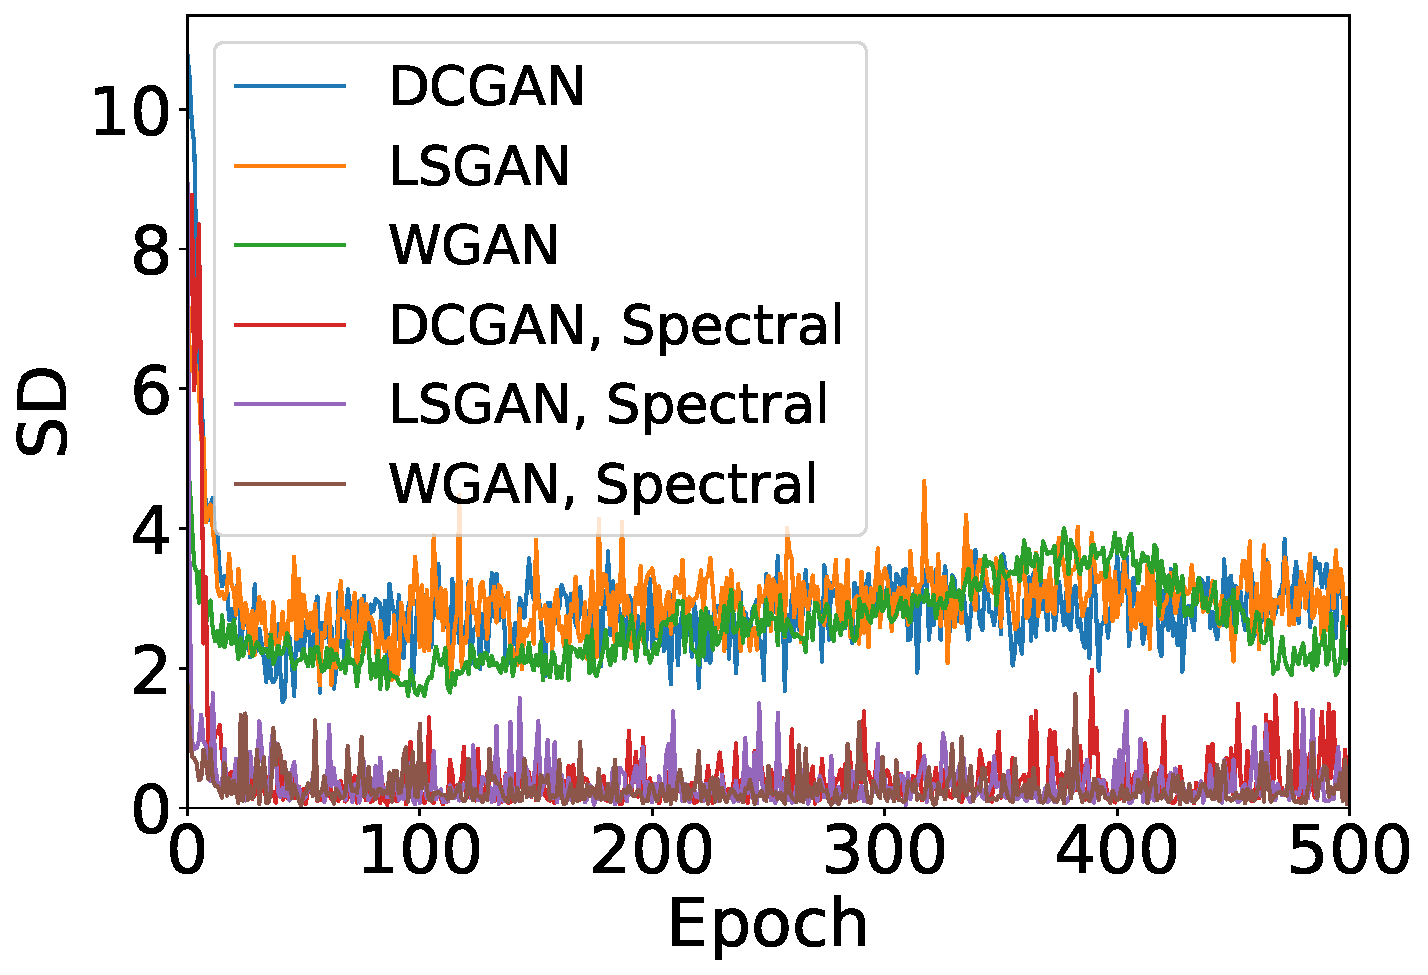
\includegraphics[width=\linewidth]{img/training_sd.pdf}
        \caption{
           With the proposed discriminator $D_F$, the spectral difference is considerably reduced.
        }
        \label{fig:detection}
    \end{subfigure}
    \caption{
        FID and SD with our models trained on FFHQ64.
        \emph{Spectral} indicates that $D_F$ was used, and omitted otherwise.
    }
    \label{fig:cloaking}
\end{figure}
\begin{figure*}[ht]
% \scriptsize
\tiny
\begin{tabular}{@{\hspace{0cm}}c@{\hspace{0cm}}c@{}c@{}c@{}c@{}c@{}c@{}c@{}}
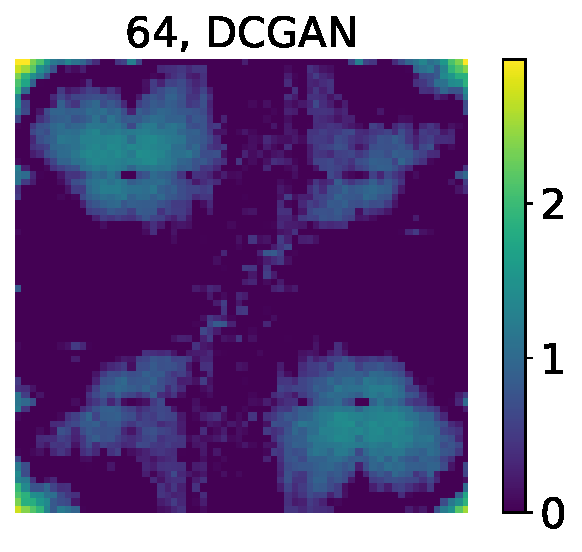
\includegraphics[width=0.125\linewidth]{img/img_2/Spectrum_64_DCGAN.pdf}&
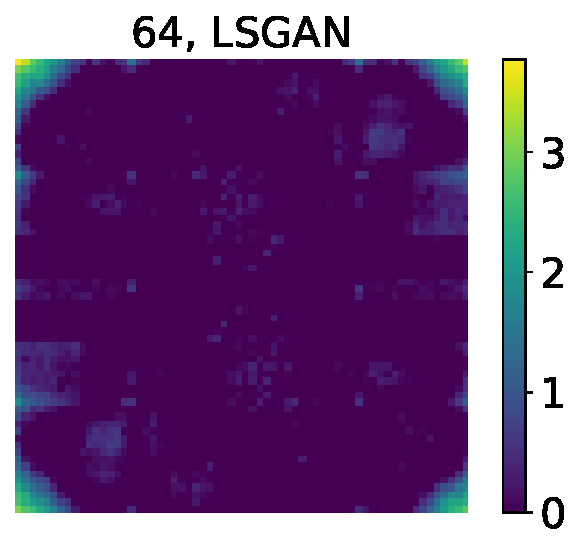
\includegraphics[width=0.125\linewidth]{img/img_2/Spectrum_64_LSGAN.pdf}&
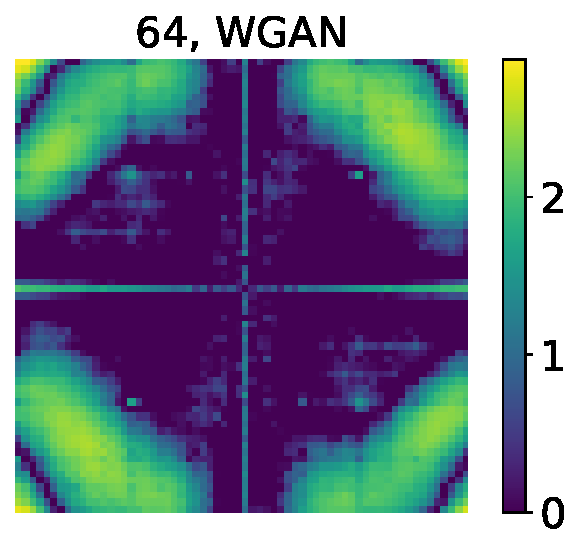
\includegraphics[width=0.125\linewidth]{img/img_2/Spectrum_64_WGAN.pdf}&
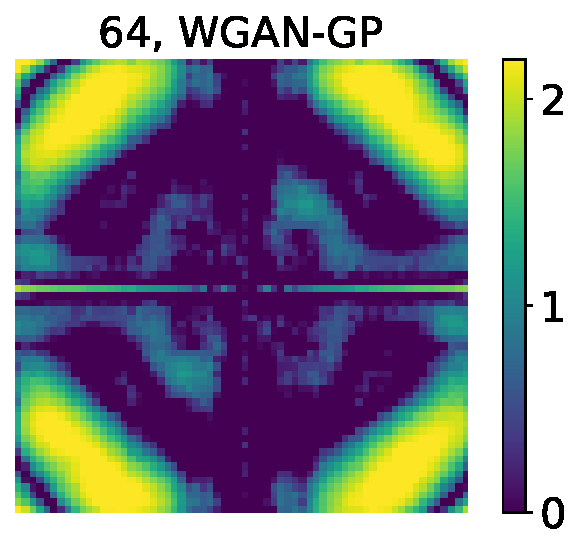
\includegraphics[width=0.125\linewidth]{img/img_2/Spectrum_64_WGAN-GP_FID.pdf}&
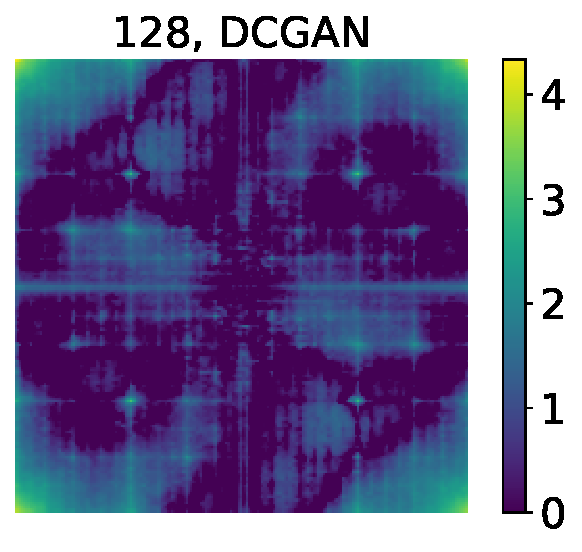
\includegraphics[width=0.125\linewidth]{img/img_2/Spectrum_128_DCGAN.pdf}&
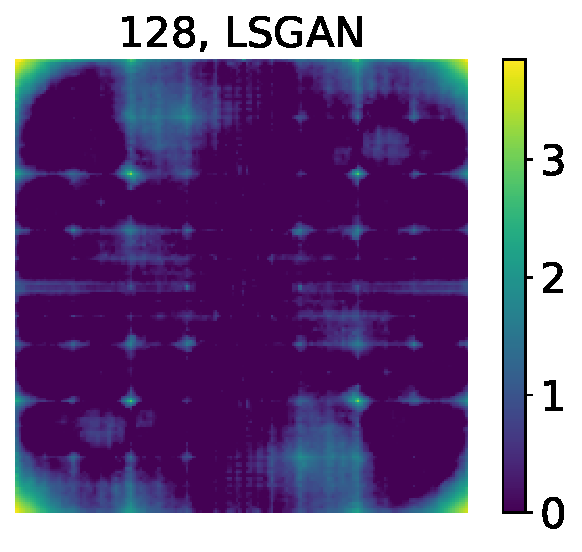
\includegraphics[width=0.125\linewidth]{img/img_2/Spectrum_128_LSGAN.pdf}&
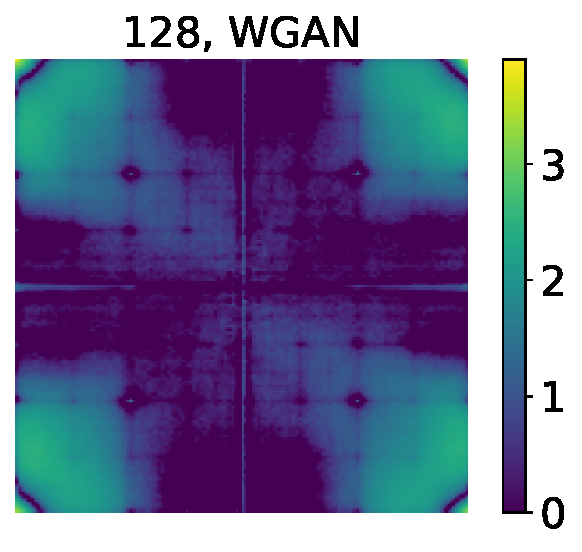
\includegraphics[width=0.125\linewidth]{img/img_2/Spectrum_128_WGAN_mix.pdf}&
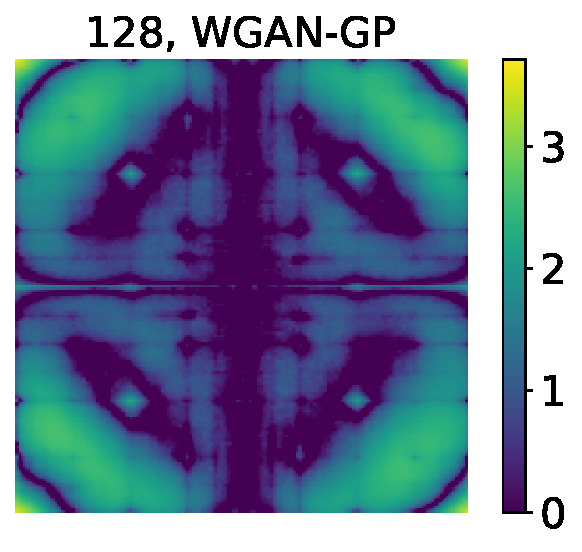
\includegraphics[width=0.125\linewidth]{img/img_2/Spectrum_128_WGAN-GP_mix.pdf}\\
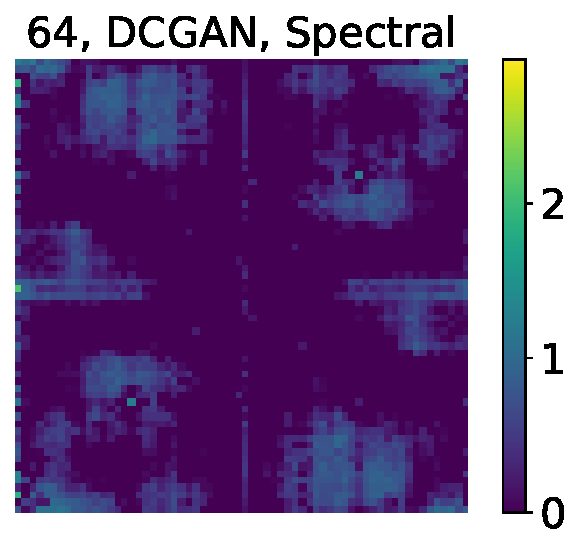
\includegraphics[width=0.125\linewidth]{img/img_2/Spectrum_64_DCGAN_Spectral.pdf}&
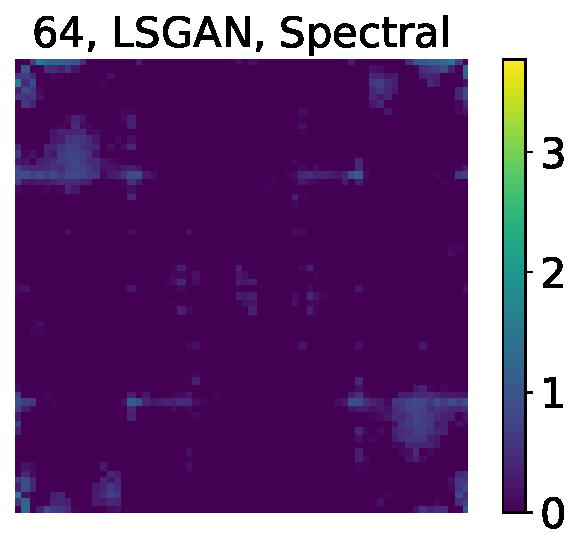
\includegraphics[width=0.125\linewidth]{img/img_2/Spectrum_64_LSGAN_Spectral.pdf}&
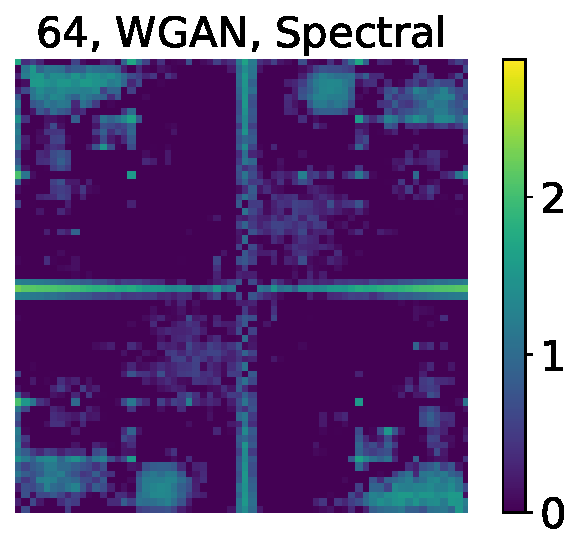
\includegraphics[width=0.125\linewidth]{img/img_2/Spectrum_64_WGAN_Spectral.pdf}&
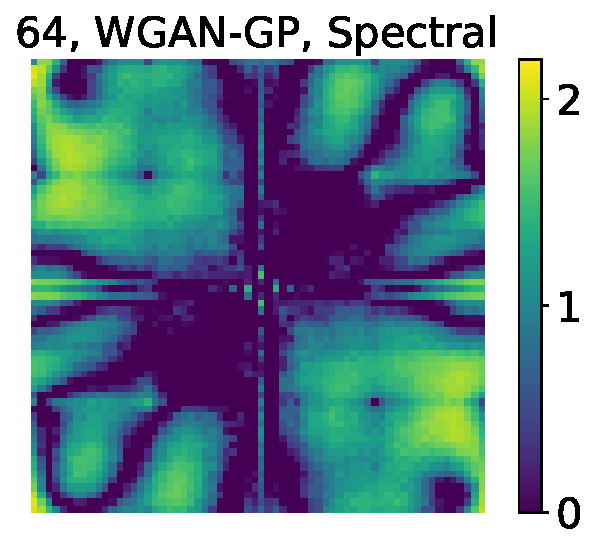
\includegraphics[width=0.125\linewidth]{img/img_2/Spectrum_64_WGAN-GP_Spectral_mix.pdf}&
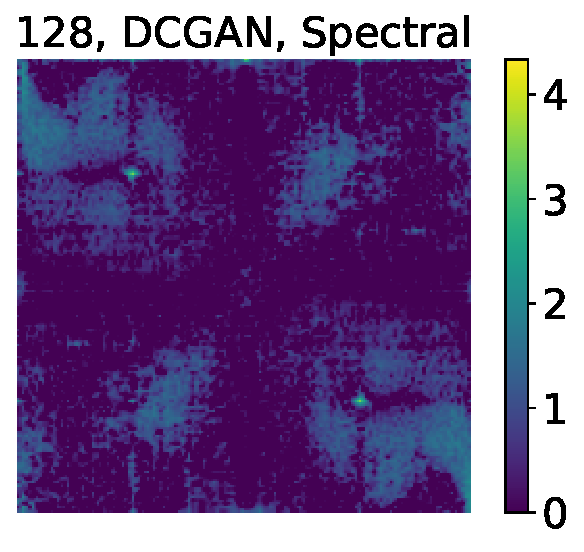
\includegraphics[width=0.125\linewidth]{img/img_2/Spectrum_128_DCGAN_Spectral.pdf}&
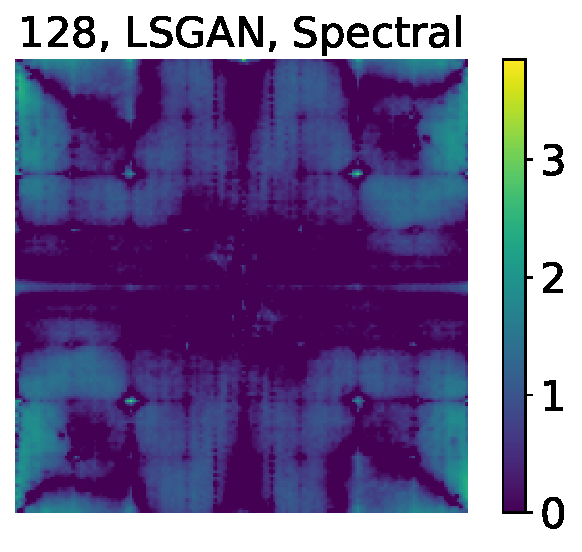
\includegraphics[width=0.125\linewidth]{img/img_2/Spectrum_128_LSGAN_Spectral.pdf}&
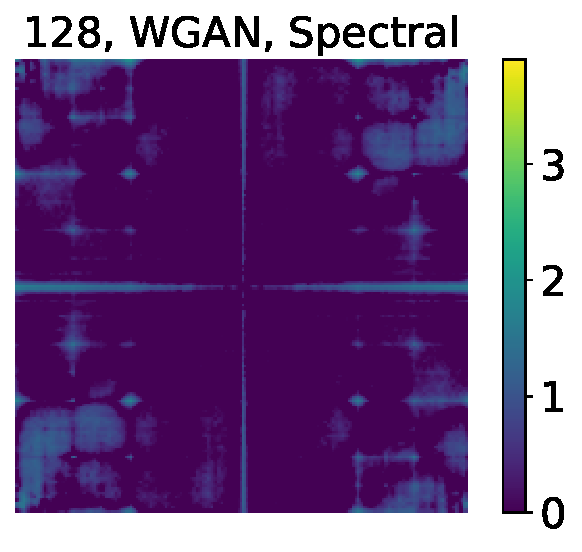
\includegraphics[width=0.125\linewidth]{img/img_2/Spectrum_128_WGAN_Spectral_SL.pdf}&
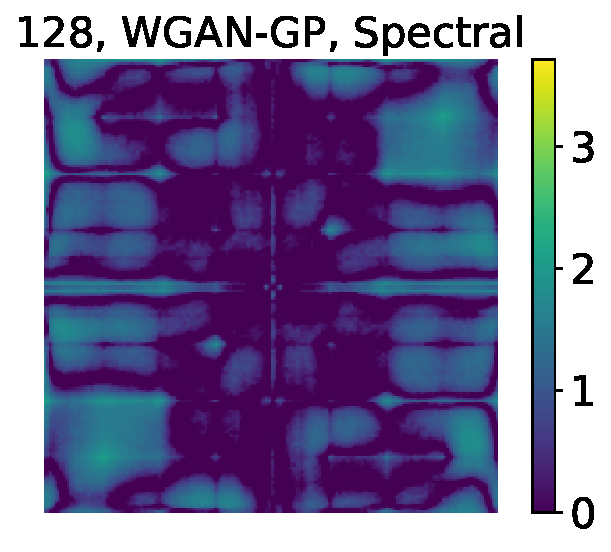
\includegraphics[width=0.125\linewidth]{img/img_2/Spectrum_128_WGAN-GP_Spectral_SL.pdf}\\
% DCGAN $64\times64$ & LSGAN $64\times64$ & WGAN $64\times64$ & WGAN-GP $64\times64$ & DCGAN $128\times128$ & LSGAN $128\times128$ & WGAN $128\times128$ & WGAN-GP $128\times128$
\end{tabular}
% \vspace{-0.1cm}
\caption{
        Mean absolute differences of the 2D power spectra of real and generated images. (Top) Differences for the original models. (Bottom) Differences for the models with spectral discriminator $D_F$. While the differences of the original models follow a characteristic pattern, our modified models show less specific differences and lower magnitudes.
    }
    \label{fig:spectra}
\end{figure*}
\begin{figure}[!ht]%[h!]
\scriptsize
\begin{tabular}{@{\hspace{0cm}}c@{\hspace{0cm}}c@{\hspace{0cm}}}
   % \begin{subfigure}[t]{.3\textwidth}
    %    \centering
        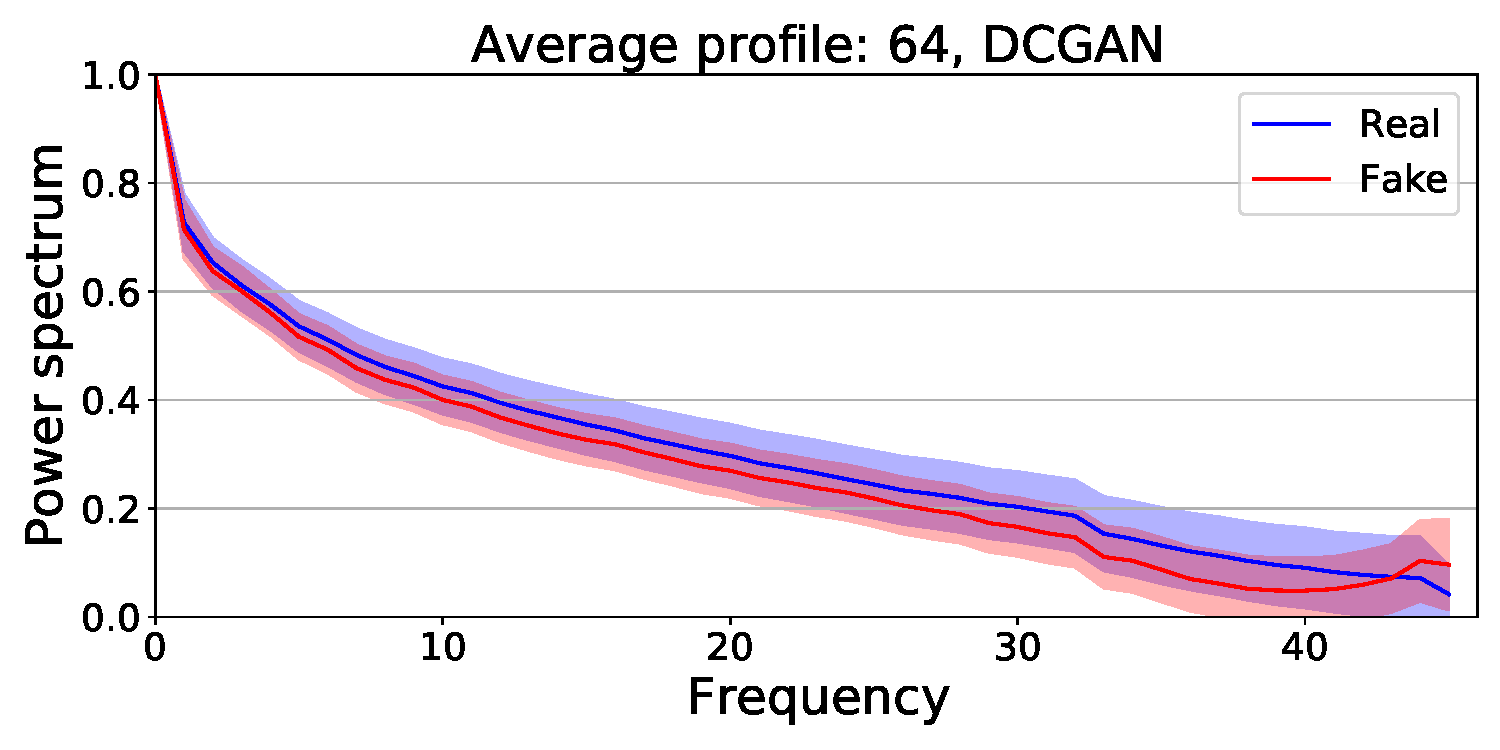
\includegraphics[width=0.49\linewidth]{img/img_2/64_DCGAN.pdf}&
        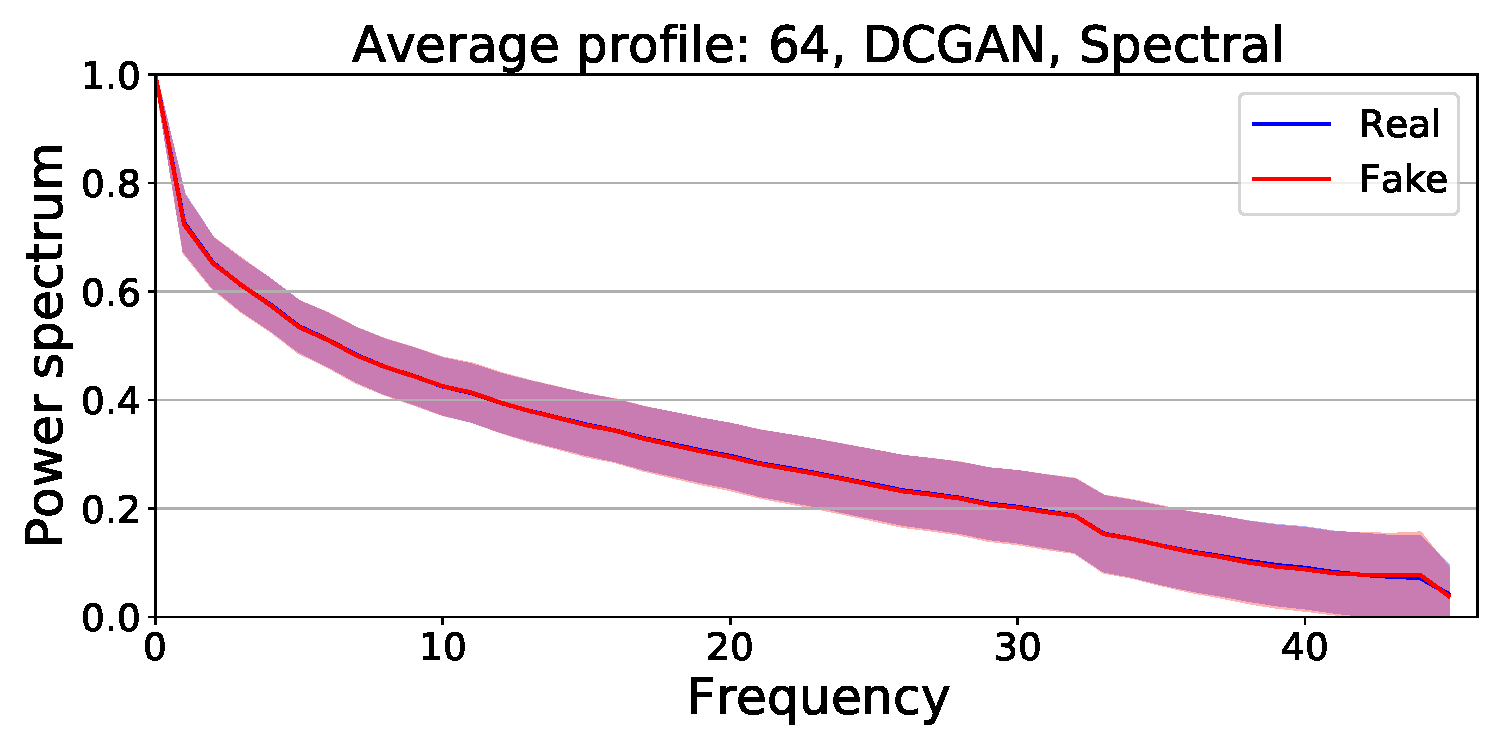
\includegraphics[width=0.49\linewidth]{img/img_2/64_DCGAN_Spectral.pdf}\\
        DCGAN& DCGAN Spectral\\
        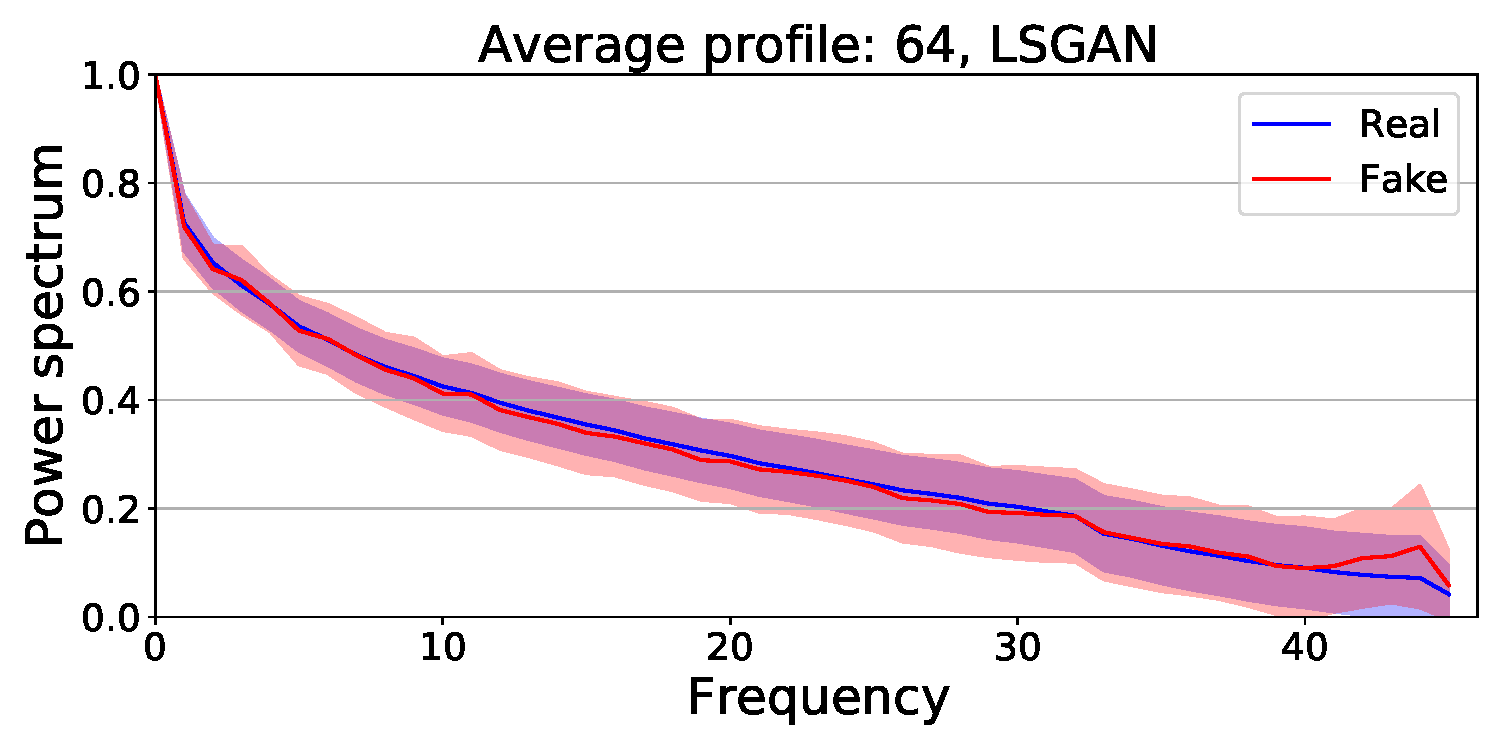
\includegraphics[width=0.49\linewidth]{img/img_2/64_LSGAN.pdf}&
        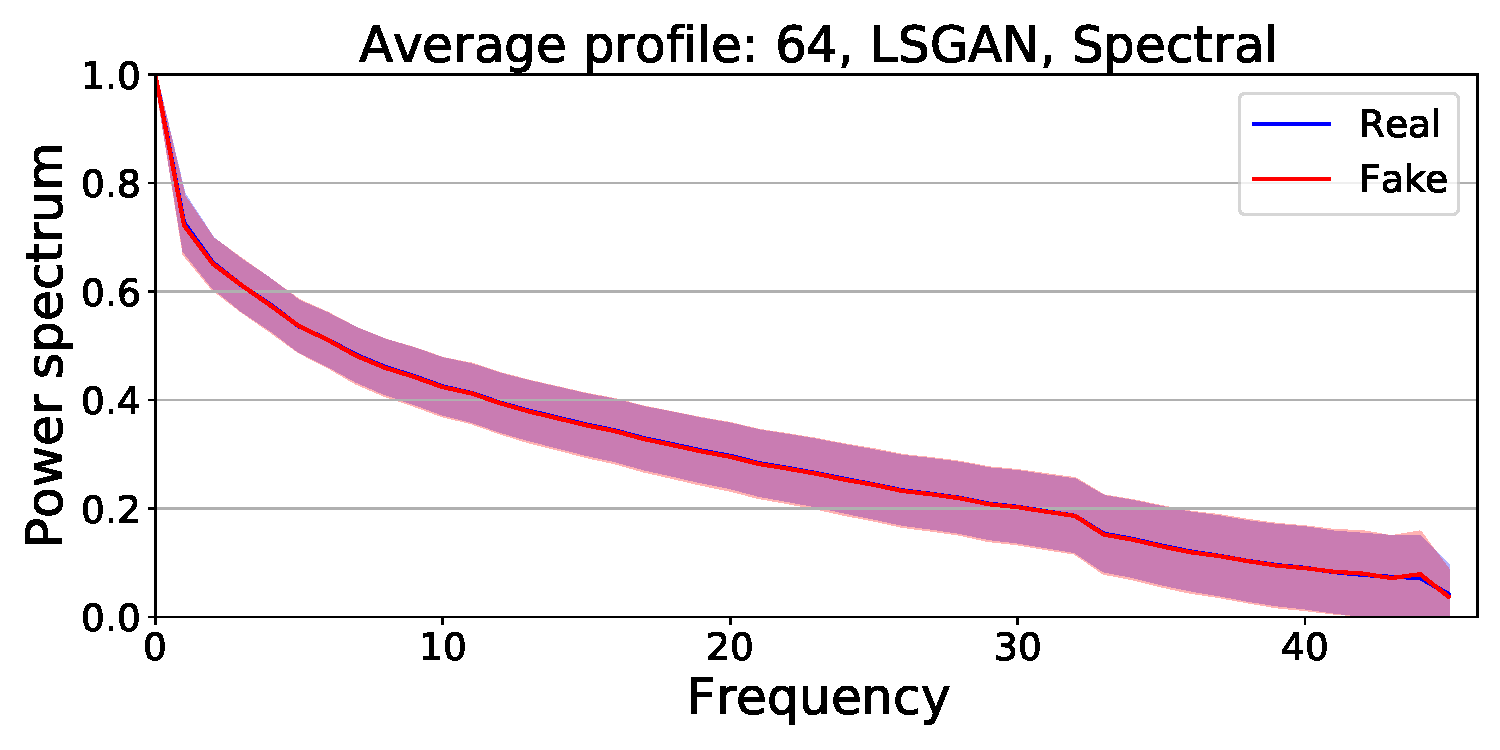
\includegraphics[width=0.49\linewidth]{img/img_2/64_LSGAN_Spectral.pdf}\\
        LSGAN& LSGAN Spectral\\
                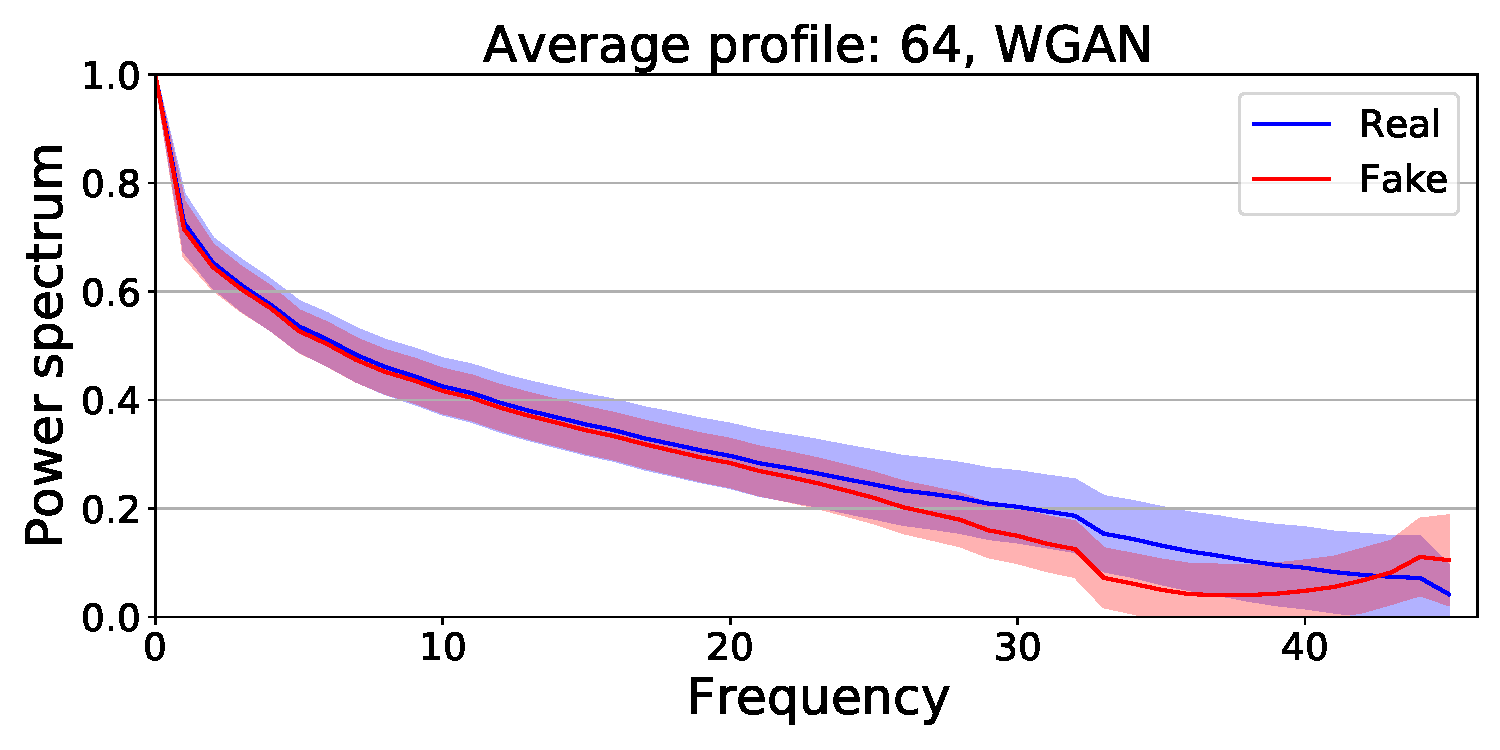
\includegraphics[width=0.49\linewidth]{img/img_2/64_WGAN.pdf}&
        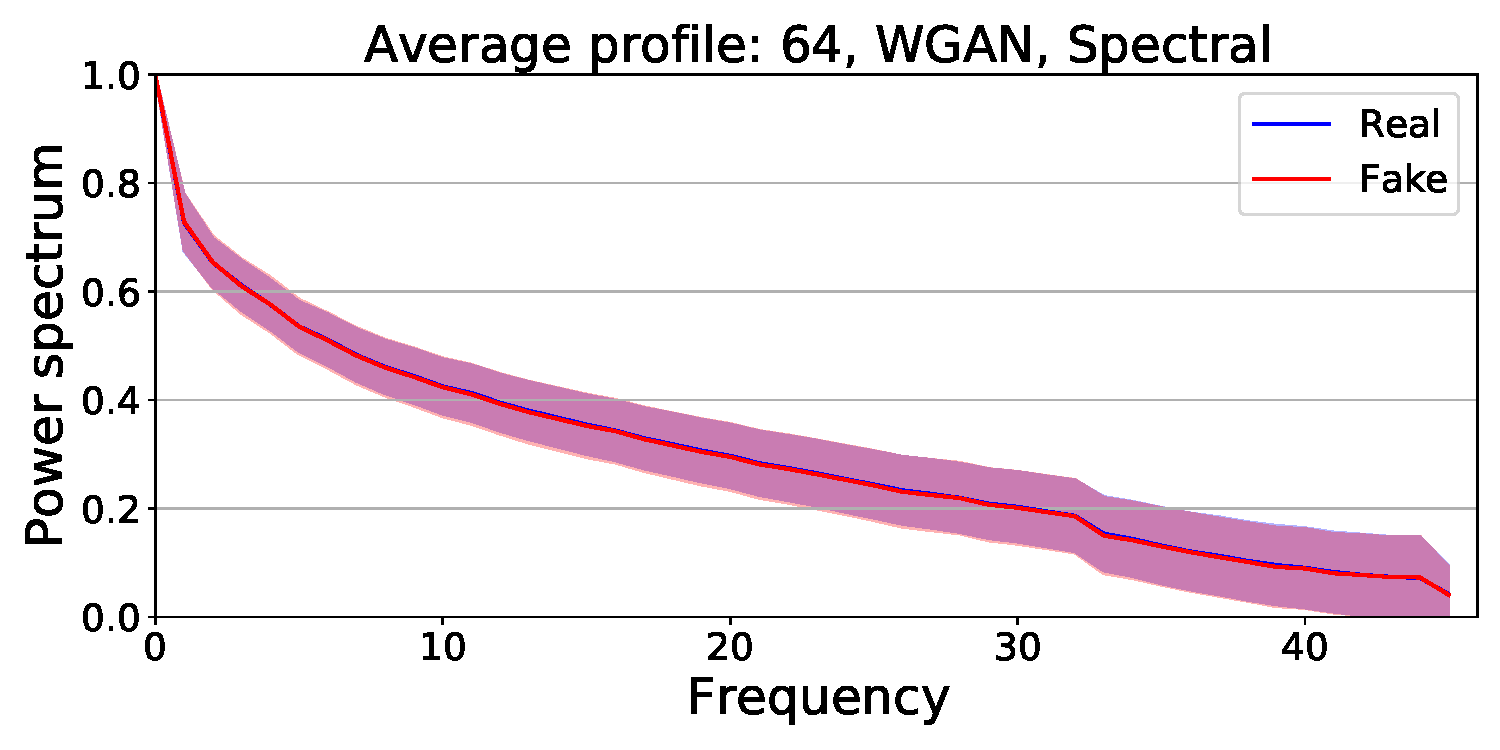
\includegraphics[width=0.49\linewidth]{img/img_2/64_WGAN_Spectral.pdf}\\
        WGAN& WGAN Spectral\\
        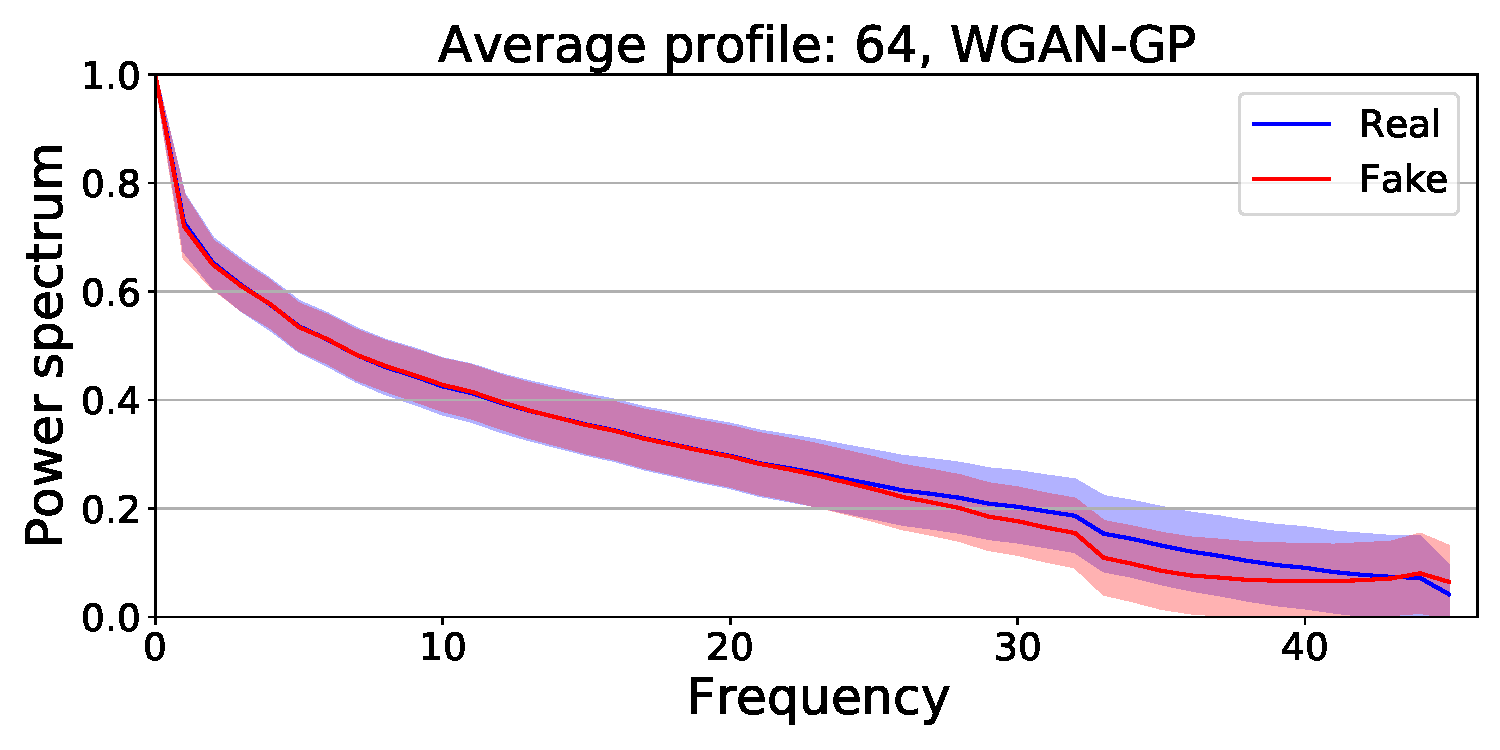
\includegraphics[width=0.49\linewidth]{img/img_2/64_WGAN-GP.pdf}&
        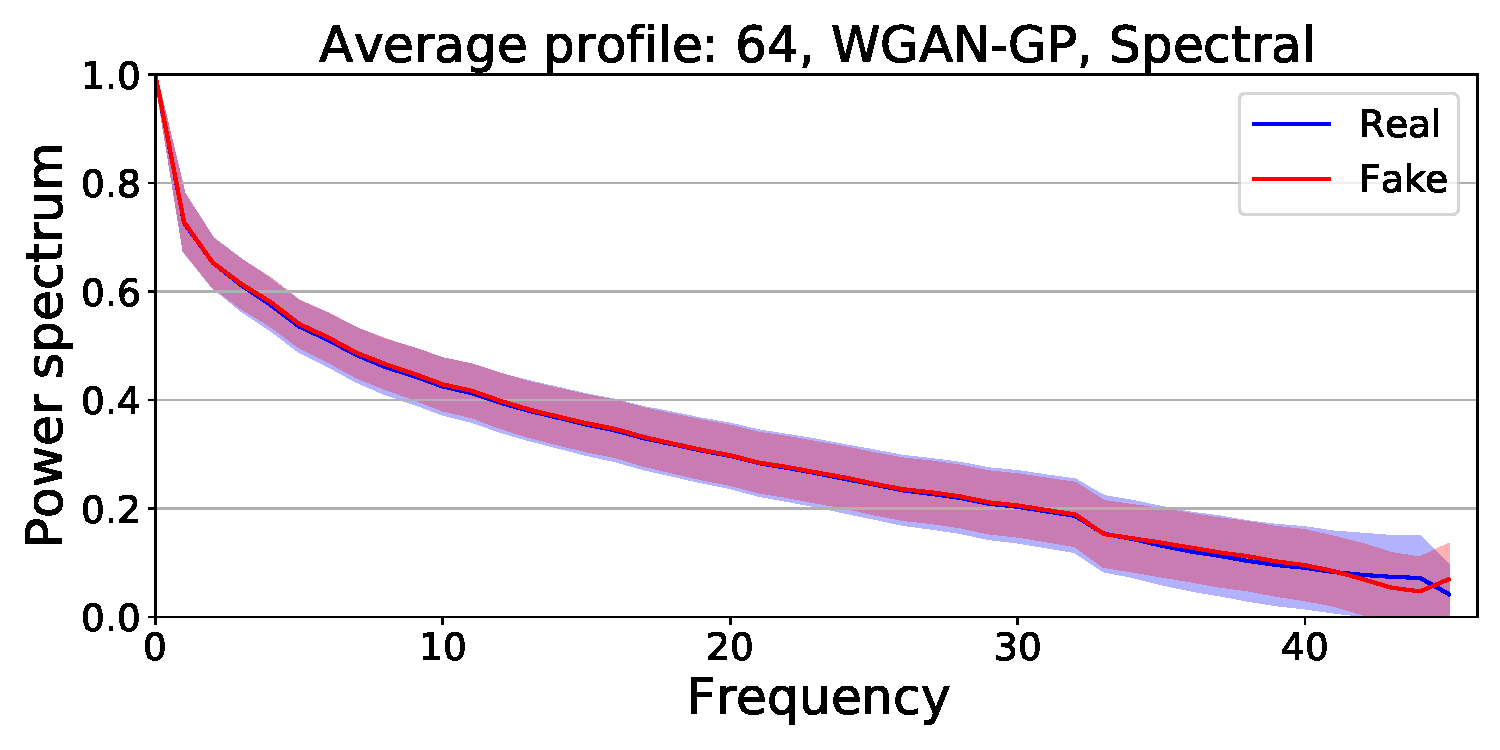
\includegraphics[width=0.49\linewidth]{img/img_2/64_WGAN-GP_Spectral.pdf}\\
        WGAN-GP& WGAN-GP Spectral\\
        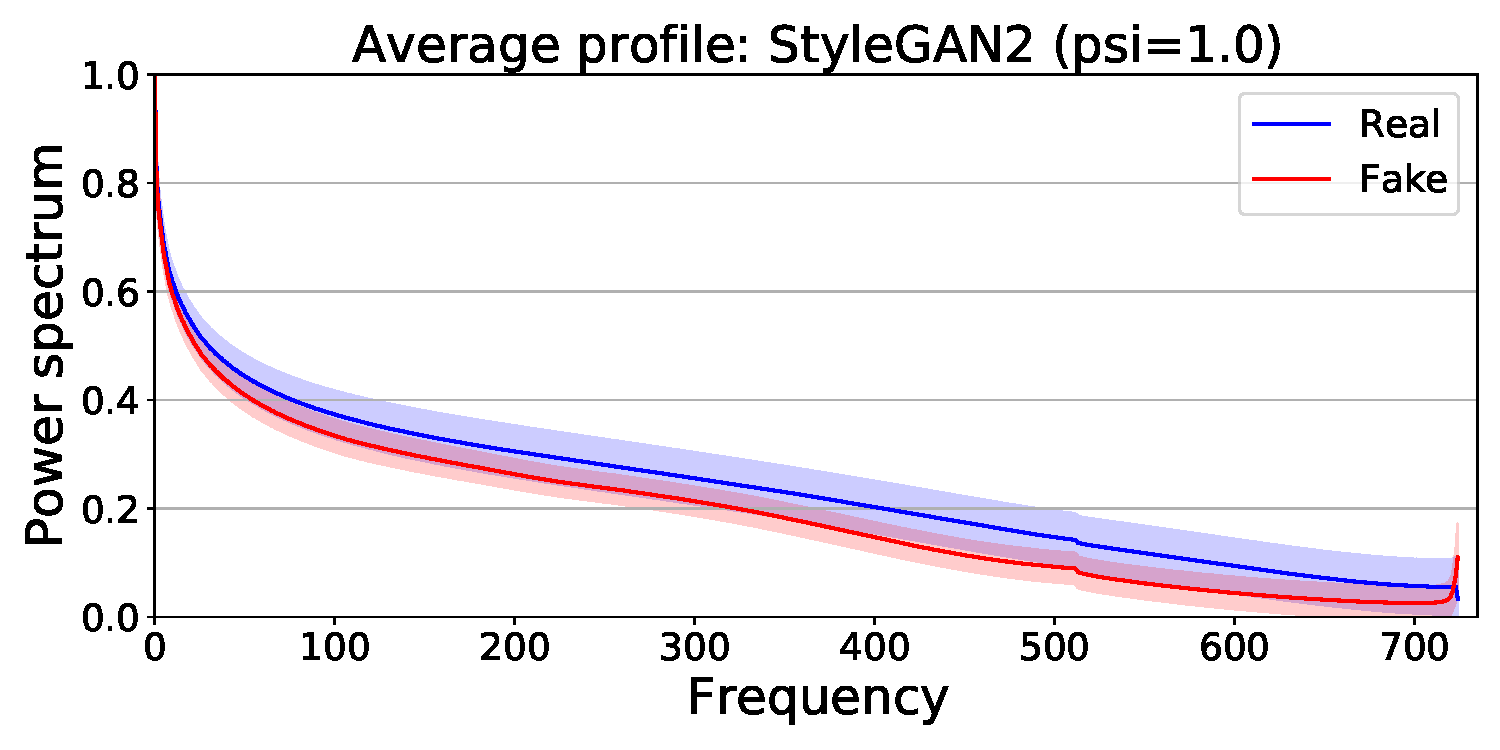
\includegraphics[width=0.49\linewidth]{img/img_2/1024_StyleGAN2.pdf}&
        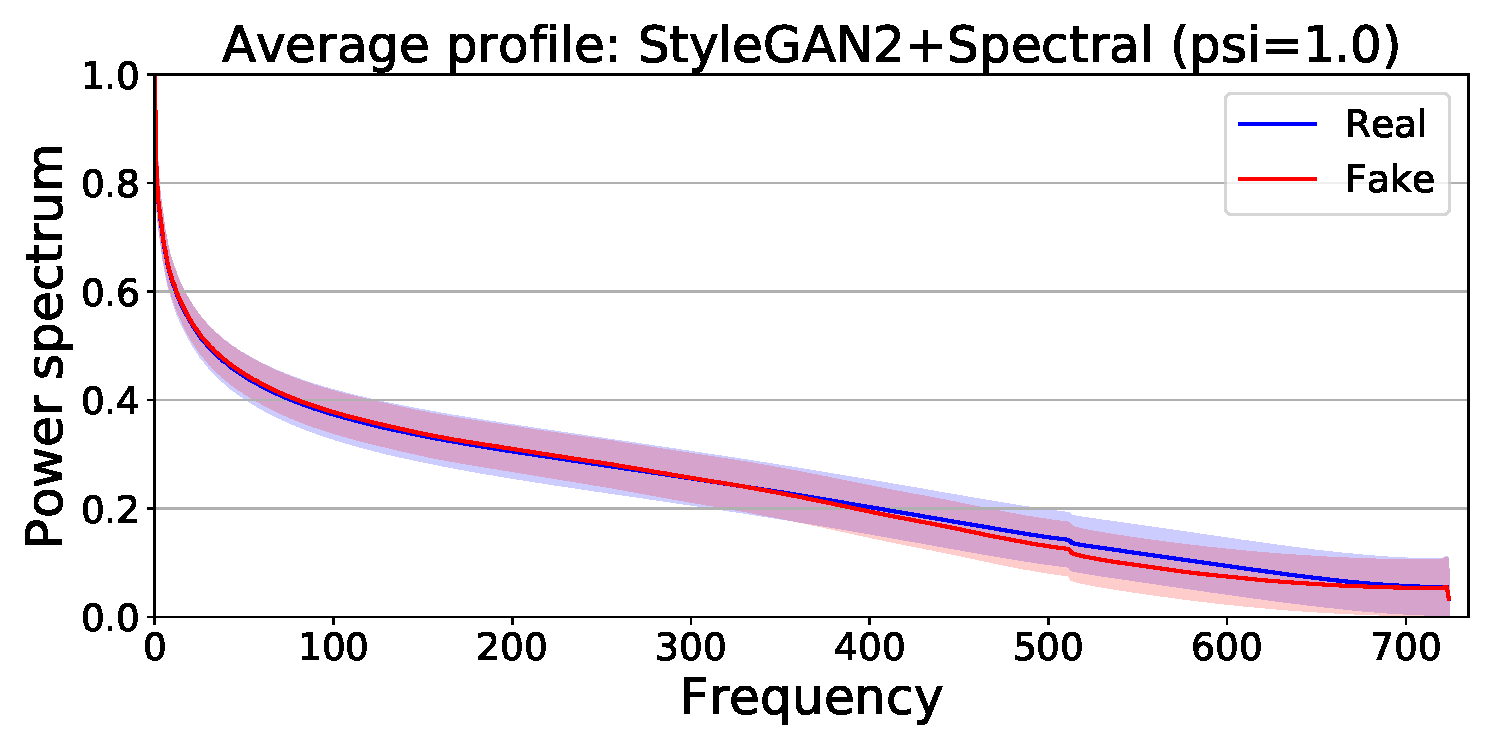
\includegraphics[width=0.49\linewidth]{img/img_2/1024_StyleGAN2_Spectral.pdf}\\
        StyleGAN2 & StyleGAN2 Spectral\\
        \iffalse
                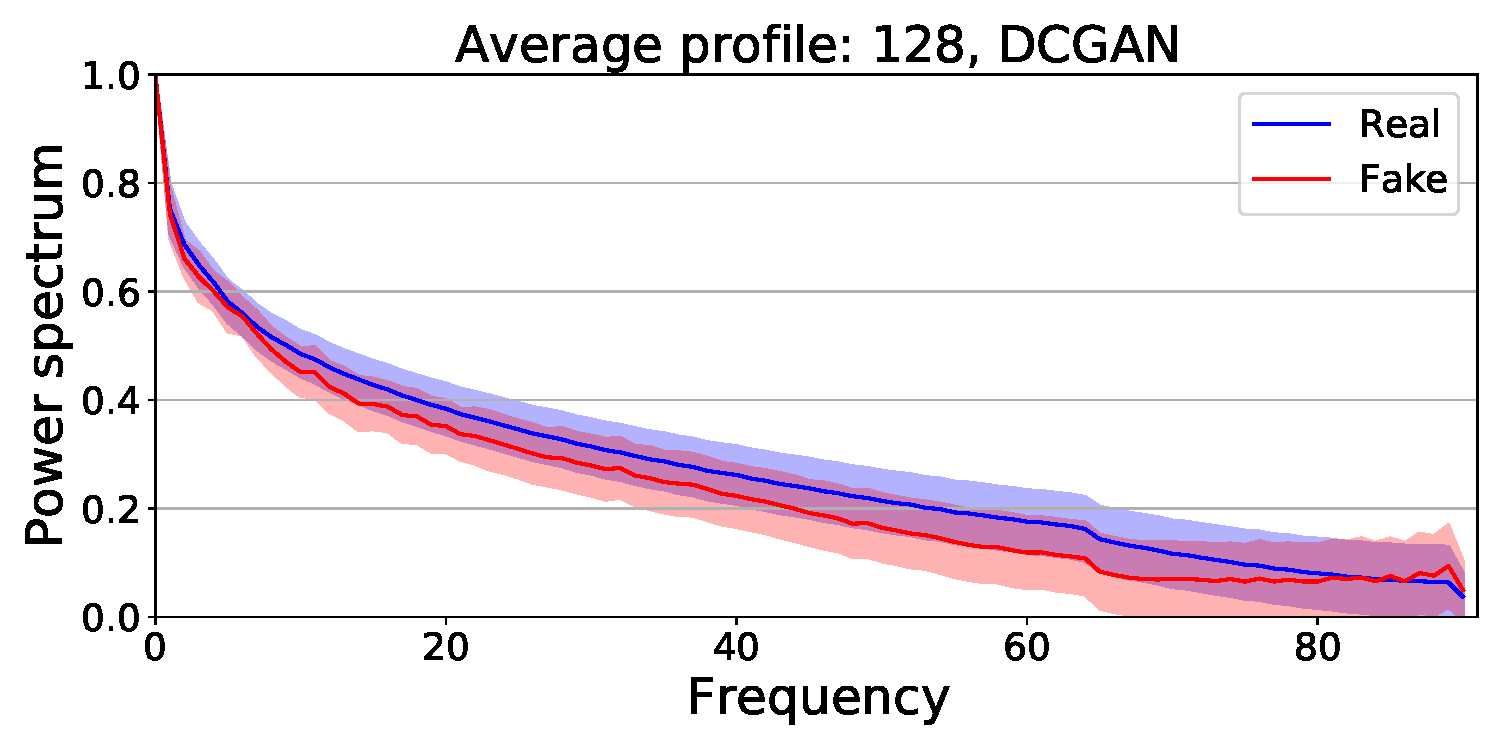
\includegraphics[width=0.49\linewidth]{img/img_2/128_DCGAN.pdf}&
                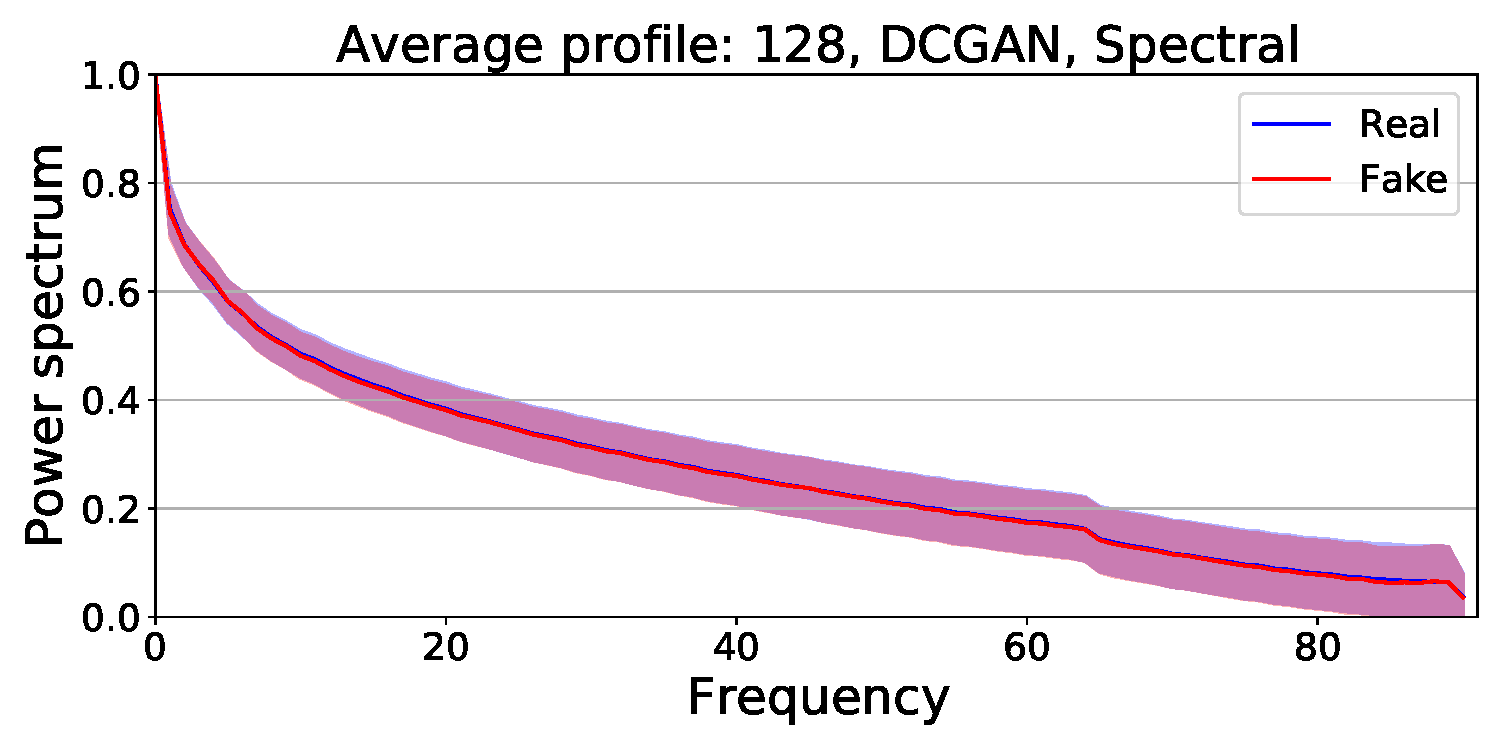
\includegraphics[width=0.49\linewidth]{img/img_2/128_DCGAN_Spectral.pdf}\\
                DCGAN& DCGAN Spectral\\
                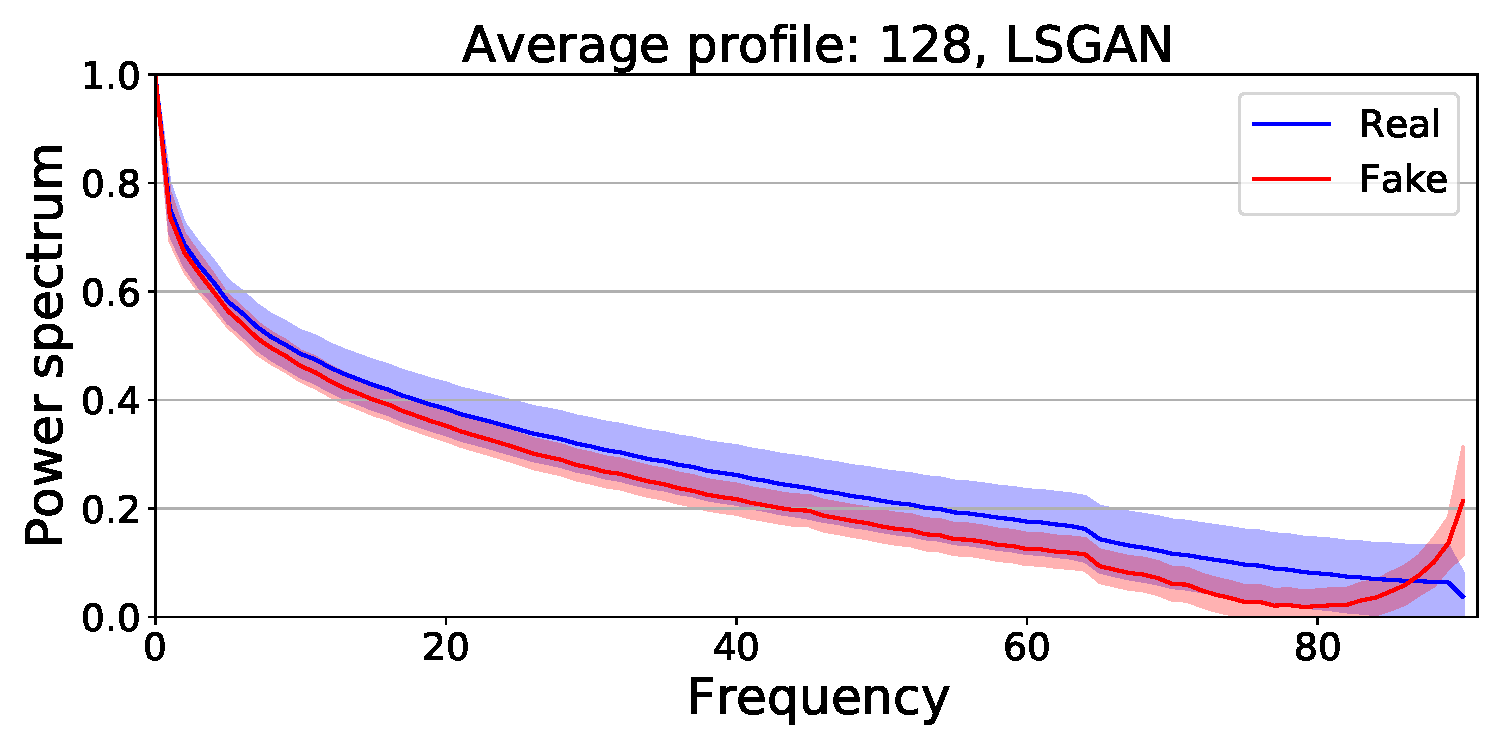
\includegraphics[width=0.49\linewidth]{img/img_2/128_LSGAN.pdf}&
                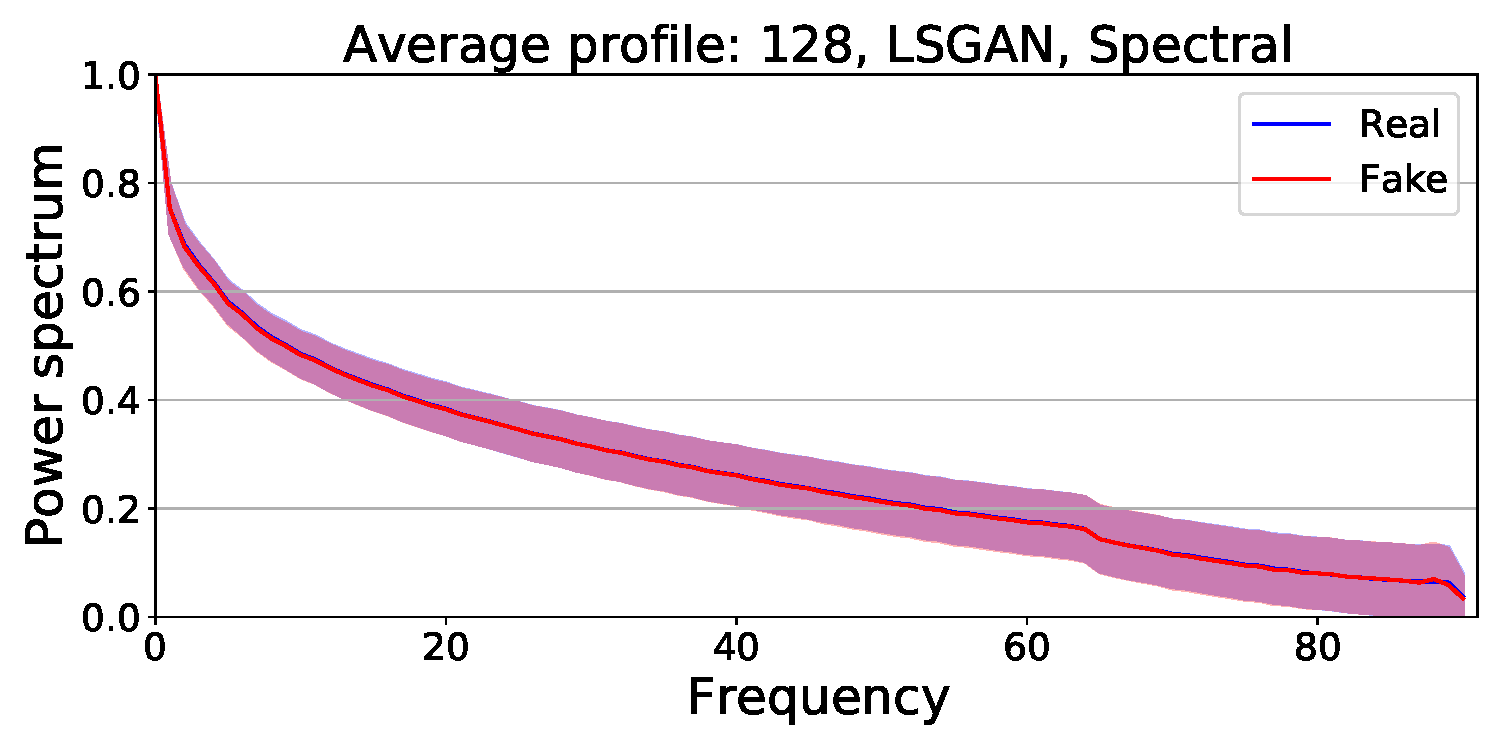
\includegraphics[width=0.49\linewidth]{img/img_2/128_LSGAN_Spectral.pdf}\\
                LSGAN& LSGAN Spectral\\
                        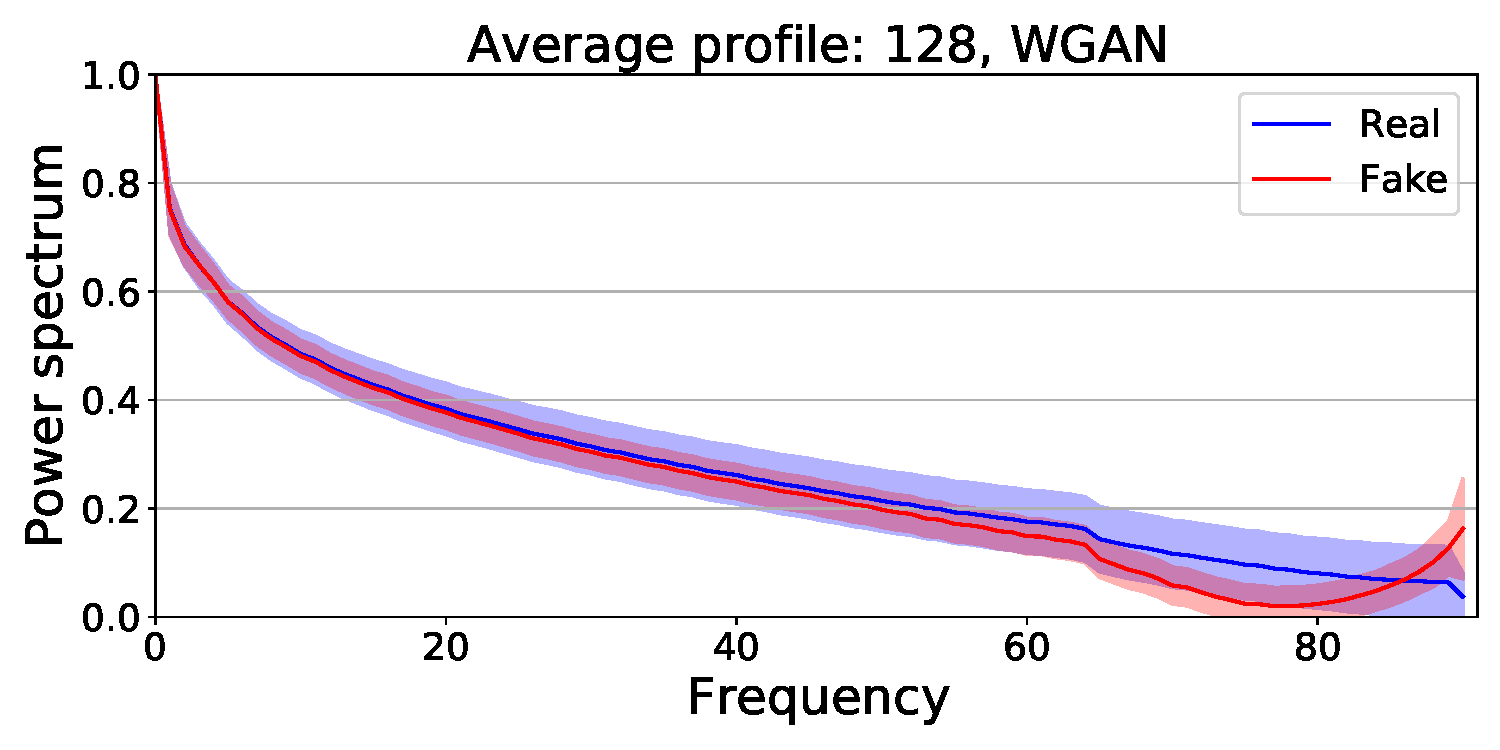
\includegraphics[width=0.49\linewidth]{img/img_2/128_WGAN.pdf}&
                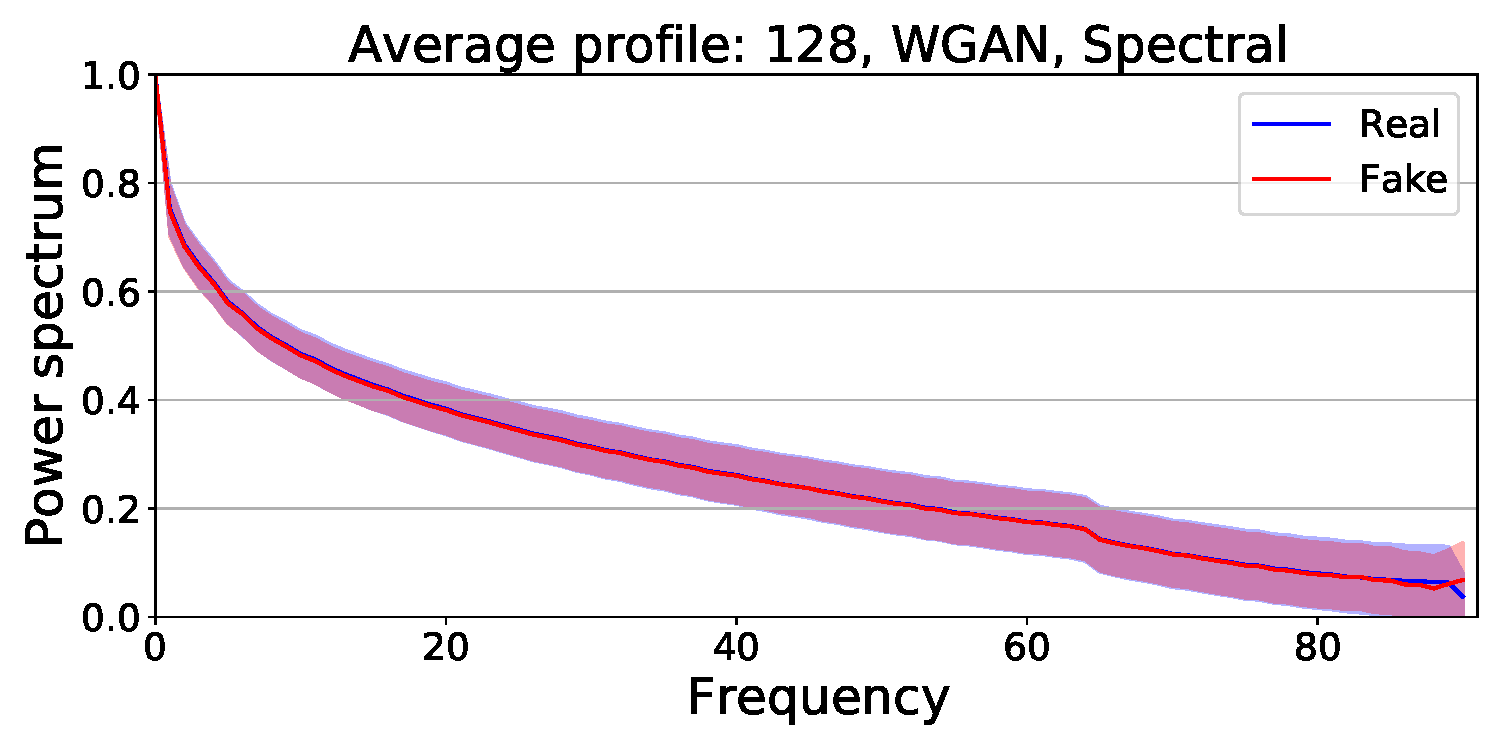
\includegraphics[width=0.49\linewidth]{img/img_2/128_WGAN_Spectral.pdf}\\
                WGAN& WGAN Spectral\\
                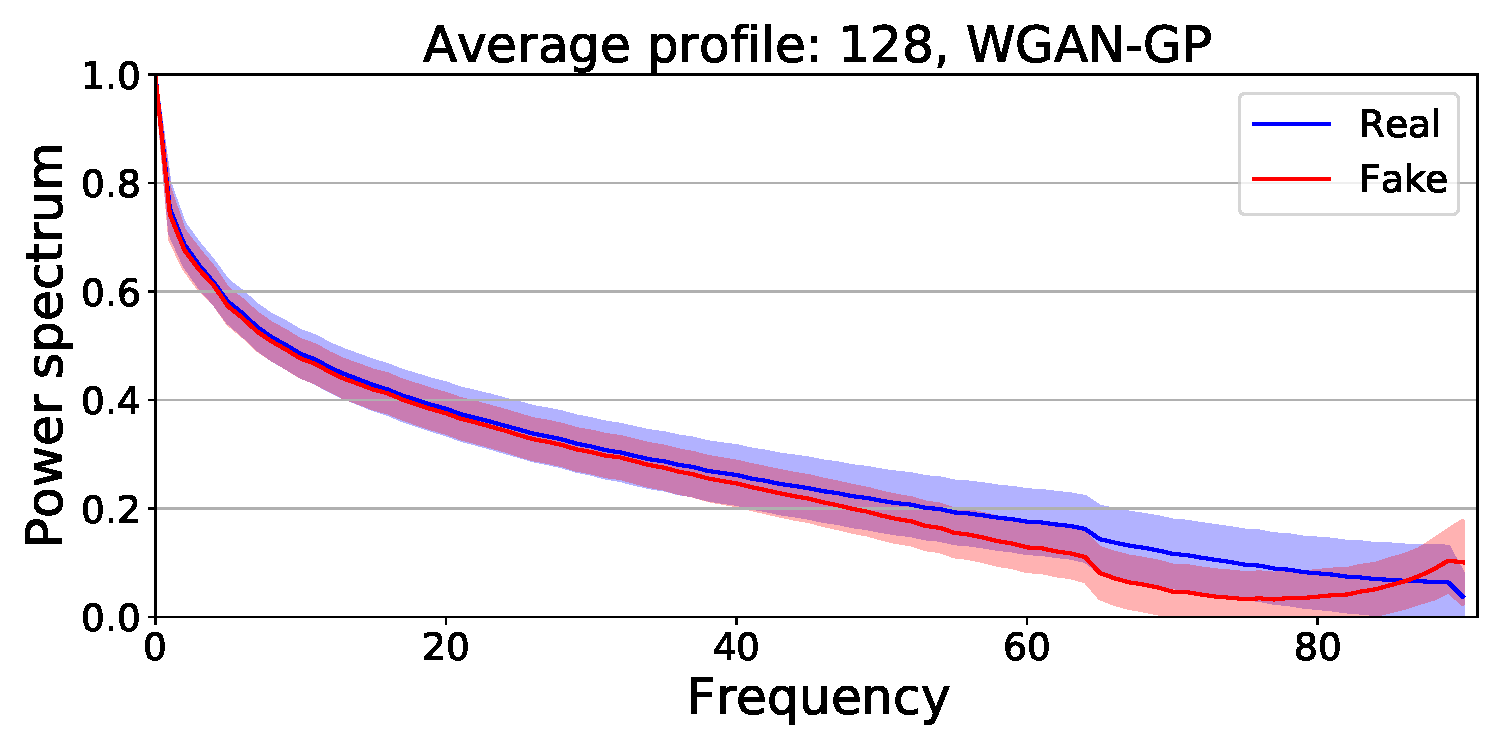
\includegraphics[width=0.49\linewidth]{img/img_2/128_WGAN-GP.pdf}&
                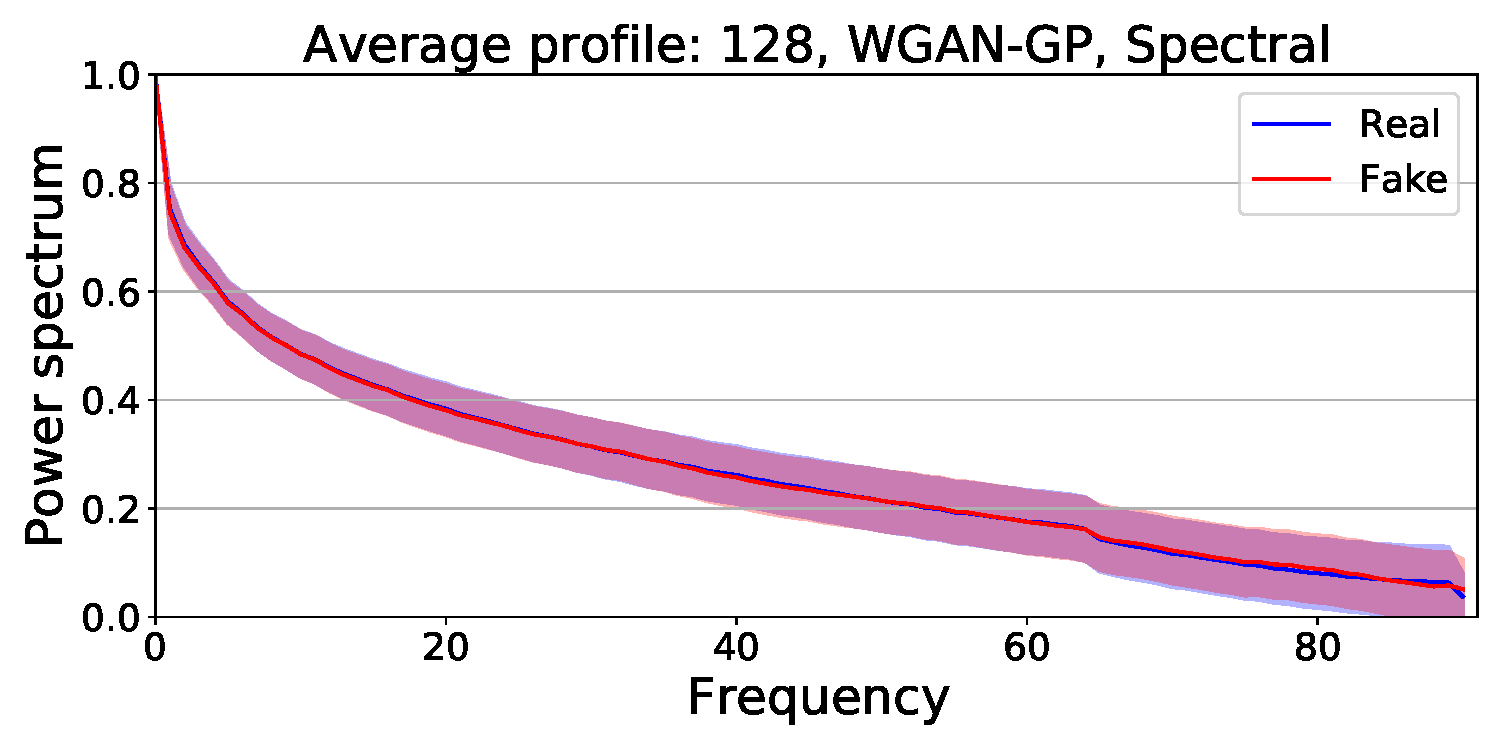
\includegraphics[width=0.49\linewidth]{img/img_2/128_WGAN-GP_Spectral.pdf}\\
                WGAN-GP& WGAN-GP Spectral\\
        \fi
        
     %   \caption{
      %      DCGAN.
      %  }
       % \label{fig:profiles}
    %\end{subfigure}
    %\hfill
    %\begin{subfigure}[t]{.3\textwidth}
    %    \centering
       
    %        LSGAN.
     %   }
     %   \label{fig:profiles}
    %\end{subfigure}
    %\hfill
    %\begin{subfigure}[t]{.3\textwidth}
     % 
        
        
        
      %  \caption{
      %      WGAN.
      %  }
    %    \label{fig:detection}
    %\end{subfigure}
    \end{tabular}
    \caption{
        Resulting spectral profiles of experiments with our models trained on FFHQ64 and StyleGAN2.
        \emph{Spectral} indicates that $D_F$ was applied. %For the respective higher resolution experiments, see the supplementary material.
        With the spectral discriminator, the mean and standard deviation of the spectral profiles fit almost perfectly.
    }
    \vspace{1em}
    \label{fig:cloaking2}
\end{figure}

The resulting FIDs over the training epochs as well as the spectral differences are displayed in Fig.~\ref{fig:profiles} and Fig.~\ref{fig:detection}, respectively. It can be seen that the proposed discriminator has a relatively small impact on the FID during training while the spectral difference is significantly reduced by our method. The effect on the spectrum can be assessed in Tab.~\ref{tab1} (left block) and in Tab.~\ref{tab1-stylegan}. For all models and resolutions, the FID is on par with the plain version without additional discriminator while the spectral difference is considerably decreased and the cloaking score increased when $D_F$ is added. The spectral regularization proposed by \citet{margret2020upconvolution} yields a significantly higher FID and lower cloaking score than the proposed approach.  %While the effect on the Wasserstein GAN is small, for DCGAN as well as for LSGAN, the proposed approach lead as well to a decreased FID score (lower is better) as to a better fit of the frequency spectra as measured by the cloaking score.

In Tab.~\ref{tab1} (right block), we further evaluate the effect of the proposed discriminator on the detectability of the generated images using recent methods from \citet{margret2020upconvolution} and \citet{Wang_2020_CVPR}. 
While \citet{margret2020upconvolution} leverage the 1D frequency spectra for the detection in a simple support vector machine (SVM) or logistic regression (LR) classifier and require retraining in every setting, \citet{Wang_2020_CVPR} train a CNN on the generated images using various data augmentations as a "universal" detector. We evaluate the method from \citet{margret2020upconvolution} in two scenarios: in the left column in Tab.~\ref{tab1} (right block) indicated with the asterix, we train on the data without spectral discriminator and evaluate in the transfer setting; in the right column, we train separately for every setting.
As can be seen, the detection is almost random in the transfer setting for the regularization approach by \citet{margret2020upconvolution} as well as for our approach in all tested GAN settings and resolutions while the generated images from \cite{margret2020upconvolution} can still be detected with about 80\% accuracy when a model is trained specifically on this data.
% Since the training behavior of the regularizer is not very stable (see supplementary material), we only evaluate it in the DCGAN setting at low resolution.
With respect to the universal detector by \citet{Wang_2020_CVPR}, both method decrease the detection accuracy significantly. This confirms that the removed frequency artifacts can in fact be perceived in the image domain and their removal is to be desired.

Figure \ref{fig:cloaking2} gives a visualization of the resulting average frequency profiles with our approach as an overlay on the average frequency of real images. With the proposed discriminator, the average frequencies fit almost perfectly. For the respective higher resolution experiments, as well as for example images generated by our approach see the supplementary material. Figure \ref{fig:spectra} shows the average differences of real and generated 2D power spectra in log-space (compare the visualization in \cite{Wang_2020_CVPR}). It can be seen that all tested GANs show specific differences. When the proposed discriminator, acting on the 1D projection of the spectra, is employed, the differences become more diffuse and have lower magnitudes. This indicates that, on average, the generated images have less perceivable sampling artifacts.  %Figure~\ref{fig:cloaking3}. Visually, they are comparable to the baseline in Fig.~\ref{fig:cloaking4}.

\iffalse
\begin{figure}
    \begin{subfigure}[t]{.3\textwidth}
        \centering
        \includegraphics[width=\linewidth]{img/profiles_DCGAN,Spectral.pdf}
        \caption{
            FID scores of our experiments.
            The resulting FID scores are similar, and the training is stable in each case.
        }
        \label{fig:profiles}
    \end{subfigure}
    \hfill
    \begin{subfigure}[t]{.3\textwidth}
        \centering
        \includegraphics[width=\linewidth]{img/profiles_LSGAN,Spectral.pdf}
        \caption{
            FID scores of our experiments.
            The resulting FID scores are similar, and the training is stable in each case.
        }
        \label{fig:profiles}
    \end{subfigure}
    \hfill
    \begin{subfigure}[t]{.3\textwidth}
        \centering
        \includegraphics[width=\linewidth]{img/profiles_WGAN,Spectral.pdf}
        \caption{
            Spectral losses of our experiments.
        }
        \label{fig:detection}
    \end{subfigure}
    \caption{
        Experiments with our models trained on FFHQ64 with different losses.
        \emph{Spectral} indicates that $D_F$ was used, and omitted otherwise.
    }
    \label{fig:cloaking}
\end{figure}
\fi

%%%%%%%%%%%%%%%%%%%%%%% 6 CONCLUSION %%%%%%%%%%%%%%%%%%

\section{Conclusion}
\label{sec:conclusion}
In this paper, we proposed an adversarial image generation approach that enables to generate images with a significantly reduced amount of spectral artifacts. The proposed method employs a simple discriminator on the 1D projections of frequency spectra of real and generated images. Thus, the generator aims to match the real data distribution not only in the image domain but also in the frequency domain. Our approach is very lightweight and allows for a stable training, as we experimentally show for different loss functions and resolutions. It generates images that can not easily be distinguished from real ones by frequency artifacts and improves, in this respect, over the recent method by~\cite{margret2020upconvolution}.




















%\pagebreak

%
% ---- Bibliography ----
%
% BibTeX users should specify bibliography style 'splncs04'.
% References will then be sorted and formatted in the correct style.
%
 %\bibliographystyle{splncs03}
 \bibliography{manuscrip}

\end{document}
